\documentclass[]{article}
\usepackage{lmodern}
\usepackage{amssymb,amsmath}
\usepackage{ifxetex,ifluatex}
\usepackage{fixltx2e} % provides \textsubscript
\ifnum 0\ifxetex 1\fi\ifluatex 1\fi=0 % if pdftex
  \usepackage[T1]{fontenc}
  \usepackage[utf8]{inputenc}
\else % if luatex or xelatex
  \ifxetex
    \usepackage{mathspec}
  \else
    \usepackage{fontspec}
  \fi
  \defaultfontfeatures{Ligatures=TeX,Scale=MatchLowercase}
\fi
% use upquote if available, for straight quotes in verbatim environments
\IfFileExists{upquote.sty}{\usepackage{upquote}}{}
% use microtype if available
\IfFileExists{microtype.sty}{%
\usepackage{microtype}
\UseMicrotypeSet[protrusion]{basicmath} % disable protrusion for tt fonts
}{}
\usepackage[margin=1in]{geometry}
\usepackage{hyperref}
\hypersetup{unicode=true,
            pdftitle={Assignment 3: K Means Clustering},
            pdfborder={0 0 0},
            breaklinks=true}
\urlstyle{same}  % don't use monospace font for urls
\usepackage{color}
\usepackage{fancyvrb}
\newcommand{\VerbBar}{|}
\newcommand{\VERB}{\Verb[commandchars=\\\{\}]}
\DefineVerbatimEnvironment{Highlighting}{Verbatim}{commandchars=\\\{\}}
% Add ',fontsize=\small' for more characters per line
\usepackage{framed}
\definecolor{shadecolor}{RGB}{248,248,248}
\newenvironment{Shaded}{\begin{snugshade}}{\end{snugshade}}
\newcommand{\AlertTok}[1]{\textcolor[rgb]{0.94,0.16,0.16}{#1}}
\newcommand{\AnnotationTok}[1]{\textcolor[rgb]{0.56,0.35,0.01}{\textbf{\textit{#1}}}}
\newcommand{\AttributeTok}[1]{\textcolor[rgb]{0.77,0.63,0.00}{#1}}
\newcommand{\BaseNTok}[1]{\textcolor[rgb]{0.00,0.00,0.81}{#1}}
\newcommand{\BuiltInTok}[1]{#1}
\newcommand{\CharTok}[1]{\textcolor[rgb]{0.31,0.60,0.02}{#1}}
\newcommand{\CommentTok}[1]{\textcolor[rgb]{0.56,0.35,0.01}{\textit{#1}}}
\newcommand{\CommentVarTok}[1]{\textcolor[rgb]{0.56,0.35,0.01}{\textbf{\textit{#1}}}}
\newcommand{\ConstantTok}[1]{\textcolor[rgb]{0.00,0.00,0.00}{#1}}
\newcommand{\ControlFlowTok}[1]{\textcolor[rgb]{0.13,0.29,0.53}{\textbf{#1}}}
\newcommand{\DataTypeTok}[1]{\textcolor[rgb]{0.13,0.29,0.53}{#1}}
\newcommand{\DecValTok}[1]{\textcolor[rgb]{0.00,0.00,0.81}{#1}}
\newcommand{\DocumentationTok}[1]{\textcolor[rgb]{0.56,0.35,0.01}{\textbf{\textit{#1}}}}
\newcommand{\ErrorTok}[1]{\textcolor[rgb]{0.64,0.00,0.00}{\textbf{#1}}}
\newcommand{\ExtensionTok}[1]{#1}
\newcommand{\FloatTok}[1]{\textcolor[rgb]{0.00,0.00,0.81}{#1}}
\newcommand{\FunctionTok}[1]{\textcolor[rgb]{0.00,0.00,0.00}{#1}}
\newcommand{\ImportTok}[1]{#1}
\newcommand{\InformationTok}[1]{\textcolor[rgb]{0.56,0.35,0.01}{\textbf{\textit{#1}}}}
\newcommand{\KeywordTok}[1]{\textcolor[rgb]{0.13,0.29,0.53}{\textbf{#1}}}
\newcommand{\NormalTok}[1]{#1}
\newcommand{\OperatorTok}[1]{\textcolor[rgb]{0.81,0.36,0.00}{\textbf{#1}}}
\newcommand{\OtherTok}[1]{\textcolor[rgb]{0.56,0.35,0.01}{#1}}
\newcommand{\PreprocessorTok}[1]{\textcolor[rgb]{0.56,0.35,0.01}{\textit{#1}}}
\newcommand{\RegionMarkerTok}[1]{#1}
\newcommand{\SpecialCharTok}[1]{\textcolor[rgb]{0.00,0.00,0.00}{#1}}
\newcommand{\SpecialStringTok}[1]{\textcolor[rgb]{0.31,0.60,0.02}{#1}}
\newcommand{\StringTok}[1]{\textcolor[rgb]{0.31,0.60,0.02}{#1}}
\newcommand{\VariableTok}[1]{\textcolor[rgb]{0.00,0.00,0.00}{#1}}
\newcommand{\VerbatimStringTok}[1]{\textcolor[rgb]{0.31,0.60,0.02}{#1}}
\newcommand{\WarningTok}[1]{\textcolor[rgb]{0.56,0.35,0.01}{\textbf{\textit{#1}}}}
\usepackage{graphicx,grffile}
\makeatletter
\def\maxwidth{\ifdim\Gin@nat@width>\linewidth\linewidth\else\Gin@nat@width\fi}
\def\maxheight{\ifdim\Gin@nat@height>\textheight\textheight\else\Gin@nat@height\fi}
\makeatother
% Scale images if necessary, so that they will not overflow the page
% margins by default, and it is still possible to overwrite the defaults
% using explicit options in \includegraphics[width, height, ...]{}
\setkeys{Gin}{width=\maxwidth,height=\maxheight,keepaspectratio}
\IfFileExists{parskip.sty}{%
\usepackage{parskip}
}{% else
\setlength{\parindent}{0pt}
\setlength{\parskip}{6pt plus 2pt minus 1pt}
}
\setlength{\emergencystretch}{3em}  % prevent overfull lines
\providecommand{\tightlist}{%
  \setlength{\itemsep}{0pt}\setlength{\parskip}{0pt}}
\setcounter{secnumdepth}{0}
% Redefines (sub)paragraphs to behave more like sections
\ifx\paragraph\undefined\else
\let\oldparagraph\paragraph
\renewcommand{\paragraph}[1]{\oldparagraph{#1}\mbox{}}
\fi
\ifx\subparagraph\undefined\else
\let\oldsubparagraph\subparagraph
\renewcommand{\subparagraph}[1]{\oldsubparagraph{#1}\mbox{}}
\fi

%%% Use protect on footnotes to avoid problems with footnotes in titles
\let\rmarkdownfootnote\footnote%
\def\footnote{\protect\rmarkdownfootnote}

%%% Change title format to be more compact
\usepackage{titling}

% Create subtitle command for use in maketitle
\providecommand{\subtitle}[1]{
  \posttitle{
    \begin{center}\large#1\end{center}
    }
}

\setlength{\droptitle}{-2em}

  \title{Assignment 3: K Means Clustering}
    \pretitle{\vspace{\droptitle}\centering\huge}
  \posttitle{\par}
    \author{}
    \preauthor{}\postauthor{}
    \date{}
    \predate{}\postdate{}
  

\begin{document}
\maketitle

In this assignment we will be applying the K-means clustering algorithm
we looked at in class. At the following link you can find a description
of K-means:

\url{https://www.cs.uic.edu/~wilkinson/Applets/cluster.html}

\begin{Shaded}
\begin{Highlighting}[]
\KeywordTok{install.packages}\NormalTok{((}\StringTok{"klaR"}\NormalTok{),}\DataTypeTok{repos =} \StringTok{"http://cran.us.r-project.org"}\NormalTok{)}
\end{Highlighting}
\end{Shaded}

\begin{verbatim}
## 
## The downloaded binary packages are in
##  /var/folders/7n/3w87168x3kv3dj0nskjj52r80000gp/T//RtmpPI5jQH/downloaded_packages
\end{verbatim}

\begin{Shaded}
\begin{Highlighting}[]
\KeywordTok{library}\NormalTok{(}\StringTok{"cluster"}\NormalTok{)}
\KeywordTok{library}\NormalTok{(}\StringTok{"dplyr"}\NormalTok{)}
\end{Highlighting}
\end{Shaded}

\begin{verbatim}
## 
## Attaching package: 'dplyr'
\end{verbatim}

\begin{verbatim}
## The following objects are masked from 'package:stats':
## 
##     filter, lag
\end{verbatim}

\begin{verbatim}
## The following objects are masked from 'package:base':
## 
##     intersect, setdiff, setequal, union
\end{verbatim}

\begin{Shaded}
\begin{Highlighting}[]
\KeywordTok{library}\NormalTok{(}\StringTok{"klaR"}\NormalTok{)}
\end{Highlighting}
\end{Shaded}

\begin{verbatim}
## Loading required package: MASS
\end{verbatim}

\begin{verbatim}
## 
## Attaching package: 'MASS'
\end{verbatim}

\begin{verbatim}
## The following object is masked from 'package:dplyr':
## 
##     select
\end{verbatim}

\begin{Shaded}
\begin{Highlighting}[]
\KeywordTok{library}\NormalTok{(}\StringTok{"tidyverse"}\NormalTok{)}
\end{Highlighting}
\end{Shaded}

\begin{verbatim}
## -- Attaching packages ---------------------------------------------------------------------- tidyverse 1.2.1 --
\end{verbatim}

\begin{verbatim}
## v ggplot2 3.2.1     v readr   1.3.1
## v tibble  2.1.3     v purrr   0.3.2
## v tidyr   1.0.0     v stringr 1.4.0
## v ggplot2 3.2.1     v forcats 0.4.0
\end{verbatim}

\begin{verbatim}
## -- Conflicts ------------------------------------------------------------------------- tidyverse_conflicts() --
## x dplyr::filter() masks stats::filter()
## x dplyr::lag()    masks stats::lag()
## x MASS::select()  masks dplyr::select()
\end{verbatim}

Now, upload the file ``Class\_Motivation.csv'' from the Assignment 3
Repository as a data frame called ``K1''"

\begin{Shaded}
\begin{Highlighting}[]
\NormalTok{K1 <-}\StringTok{ }\KeywordTok{read.csv}\NormalTok{(}\StringTok{"~/Desktop/2019fall/core methods in edm/assignment3/Class_Motivation.csv"}\NormalTok{, }\DataTypeTok{header=}\OtherTok{TRUE}\NormalTok{)}
\NormalTok{K1}
\end{Highlighting}
\end{Shaded}

\begin{verbatim}
##          id motivation1 motivation2 motivation3 motivation4 motivation5
## 1  10005216           2           2           2           2           2
## 2  10033216           3          NA           3          NA          NA
## 3  10004216           1           2           1           2           2
## 4  10008216           1           2           1           2          NA
## 5  10026216           3          NA           3          NA          NA
## 6  10014216           2          NA           2          NA           2
## 7  10021216           2           2           2           2           2
## 8  10013216           2          NA           2          NA           1
## 9  10035216           2           3           2           3          NA
## 10 10015216           2           2           2           2           2
## 11 10031216           1           1           1           1          NA
## 12 10007216           2           1           2           1           2
## 13 10010216           2           2           2           2          NA
## 14 10020216           2           3           2           3           1
## 15 10002216           1           1           1           1           4
## 16 10011216           2           2           2           2          NA
## 17 10023216           1           1           1           1           3
## 18 10028216           1           1           1           1           1
## 19 10028216           1           1           1           1           1
## 20 10034216           3           2           3           2           2
## 21 10003216           2          NA           2          NA          NA
## 22 10029216           2           2           2           2           5
## 23 10022216           1           3           1           3          NA
## 24 10006216           1           1           1           1          NA
## 25 10009216           1           1           1           1           2
## 26 10018216           1           2           1           2           4
## 27 10018216           1           2           1           2           3
## 28 10018216           1           2           1           2           4
## 29 10018216           1           2           1           2           3
## 30 10018216           1           2           1           2           4
## 31 10018216           1           2           1           2           3
## 32 10018216           1           2           1           2           4
## 33 10018216           1           2           1           2           3
## 34 10027216           1           1           1           1           1
## 35 10025216           2           2           2           2           2
## 36 10019216           1          NA           1          NA          NA
## 37 10032216           3          NA           3          NA          NA
## 38 10017216           3          NA           3          NA           3
\end{verbatim}

This file contains the self-reported motivation scores for a class over
five weeks. We are going to look for patterns in motivation over this
time and sort people into clusters based on those patterns.

But before we do that, we will need to manipulate the data frame into a
structure that can be analyzed by our clustering algorithm.

The algorithm will treat each row as a value belonging to a person, so
we need to remove the id variable.

\begin{Shaded}
\begin{Highlighting}[]
\NormalTok{    K2 <-}\StringTok{ }\NormalTok{dplyr}\OperatorTok{::}\KeywordTok{select}\NormalTok{(K1, }\DecValTok{2}\OperatorTok{:}\DecValTok{6}\NormalTok{)}
\NormalTok{K2}
\end{Highlighting}
\end{Shaded}

\begin{verbatim}
##    motivation1 motivation2 motivation3 motivation4 motivation5
## 1            2           2           2           2           2
## 2            3          NA           3          NA          NA
## 3            1           2           1           2           2
## 4            1           2           1           2          NA
## 5            3          NA           3          NA          NA
## 6            2          NA           2          NA           2
## 7            2           2           2           2           2
## 8            2          NA           2          NA           1
## 9            2           3           2           3          NA
## 10           2           2           2           2           2
## 11           1           1           1           1          NA
## 12           2           1           2           1           2
## 13           2           2           2           2          NA
## 14           2           3           2           3           1
## 15           1           1           1           1           4
## 16           2           2           2           2          NA
## 17           1           1           1           1           3
## 18           1           1           1           1           1
## 19           1           1           1           1           1
## 20           3           2           3           2           2
## 21           2          NA           2          NA          NA
## 22           2           2           2           2           5
## 23           1           3           1           3          NA
## 24           1           1           1           1          NA
## 25           1           1           1           1           2
## 26           1           2           1           2           4
## 27           1           2           1           2           3
## 28           1           2           1           2           4
## 29           1           2           1           2           3
## 30           1           2           1           2           4
## 31           1           2           1           2           3
## 32           1           2           1           2           4
## 33           1           2           1           2           3
## 34           1           1           1           1           1
## 35           2           2           2           2           2
## 36           1          NA           1          NA          NA
## 37           3          NA           3          NA          NA
## 38           3          NA           3          NA           3
\end{verbatim}

It is important to think about the meaning of missing values when
clustering. We could treat them as having meaning or we could remove
those people who have them. Neither option is ideal. What problems do
you foresee if we recode or remove these values? Write your answers
below:

We will remove people with missing values for this assignment, but keep
in mind the issues that you have identified.

\begin{Shaded}
\begin{Highlighting}[]
\NormalTok{K3 <-}\StringTok{ }\KeywordTok{na.omit}\NormalTok{(K2) }\CommentTok{#This command create a data frame with only those people with no missing values. It "omits" all rows with missing values, also known as a "listwise deletion". EG - It runs down the list deleting rows as it goes.}
\NormalTok{K3}
\end{Highlighting}
\end{Shaded}

\begin{verbatim}
##    motivation1 motivation2 motivation3 motivation4 motivation5
## 1            2           2           2           2           2
## 3            1           2           1           2           2
## 7            2           2           2           2           2
## 10           2           2           2           2           2
## 12           2           1           2           1           2
## 14           2           3           2           3           1
## 15           1           1           1           1           4
## 17           1           1           1           1           3
## 18           1           1           1           1           1
## 19           1           1           1           1           1
## 20           3           2           3           2           2
## 22           2           2           2           2           5
## 25           1           1           1           1           2
## 26           1           2           1           2           4
## 27           1           2           1           2           3
## 28           1           2           1           2           4
## 29           1           2           1           2           3
## 30           1           2           1           2           4
## 31           1           2           1           2           3
## 32           1           2           1           2           4
## 33           1           2           1           2           3
## 34           1           1           1           1           1
## 35           2           2           2           2           2
\end{verbatim}

Another pre-processing step used in K-means is to standardize the values
so that they have the same range. We do this because we want to treat
each week as equally important - if we do not standardise then the week
with the largest range will have the greatest impact on which clusters
are formed. We standardise the values by using the ``scale()'' command.

\begin{Shaded}
\begin{Highlighting}[]
\NormalTok{K3 <-}\KeywordTok{scale}\NormalTok{(K3)}
\NormalTok{K3}
\end{Highlighting}
\end{Shaded}

\begin{verbatim}
##    motivation1 motivation2 motivation3 motivation4 motivation5
## 1    1.0440258   0.4823561   1.0440258   0.4823561  -0.5258485
## 3   -0.6711594   0.4823561  -0.6711594   0.4823561  -0.5258485
## 7    1.0440258   0.4823561   1.0440258   0.4823561  -0.5258485
## 10   1.0440258   0.4823561   1.0440258   0.4823561  -0.5258485
## 12   1.0440258  -1.3666757   1.0440258  -1.3666757  -0.5258485
## 14   1.0440258   2.3313880   1.0440258   2.3313880  -1.3897424
## 15  -0.6711594  -1.3666757  -0.6711594  -1.3666757   1.2019394
## 17  -0.6711594  -1.3666757  -0.6711594  -1.3666757   0.3380454
## 18  -0.6711594  -1.3666757  -0.6711594  -1.3666757  -1.3897424
## 19  -0.6711594  -1.3666757  -0.6711594  -1.3666757  -1.3897424
## 20   2.7592111   0.4823561   2.7592111   0.4823561  -0.5258485
## 22   1.0440258   0.4823561   1.0440258   0.4823561   2.0658333
## 25  -0.6711594  -1.3666757  -0.6711594  -1.3666757  -0.5258485
## 26  -0.6711594   0.4823561  -0.6711594   0.4823561   1.2019394
## 27  -0.6711594   0.4823561  -0.6711594   0.4823561   0.3380454
## 28  -0.6711594   0.4823561  -0.6711594   0.4823561   1.2019394
## 29  -0.6711594   0.4823561  -0.6711594   0.4823561   0.3380454
## 30  -0.6711594   0.4823561  -0.6711594   0.4823561   1.2019394
## 31  -0.6711594   0.4823561  -0.6711594   0.4823561   0.3380454
## 32  -0.6711594   0.4823561  -0.6711594   0.4823561   1.2019394
## 33  -0.6711594   0.4823561  -0.6711594   0.4823561   0.3380454
## 34  -0.6711594  -1.3666757  -0.6711594  -1.3666757  -1.3897424
## 35   1.0440258   0.4823561   1.0440258   0.4823561  -0.5258485
## attr(,"scaled:center")
## motivation1 motivation2 motivation3 motivation4 motivation5 
##    1.391304    1.739130    1.391304    1.739130    2.608696 
## attr(,"scaled:scale")
## motivation1 motivation2 motivation3 motivation4 motivation5 
##   0.5830274   0.5408236   0.5830274   0.5408236   1.1575495
\end{verbatim}

Now we will run the K-means clustering algorithm we talked about in
class. 1) The algorithm starts by randomly choosing some starting values
2) Associates all observations near to those values with them 3)
Calculates the mean of those clusters of values 4) Selects the
observation closest to the mean of the cluster 5) Re-associates all
observations closest to this observation 6) Continues this process until
the clusters are no longer changing

Notice that in this case we have 5 variables and in class we only had 2.
It is impossible to vizualise this process with 5 variables.

Also, we need to choose the number of clusters we think are in the data.
We will start with 2.

\begin{Shaded}
\begin{Highlighting}[]
\NormalTok{fit <-}\StringTok{ }\KeywordTok{kmeans}\NormalTok{(K3,}\DecValTok{2}\NormalTok{)}
\NormalTok{fit}
\end{Highlighting}
\end{Shaded}

\begin{verbatim}
## K-means clustering with 2 clusters of sizes 8, 15
## 
## Cluster means:
##   motivation1 motivation2 motivation3 motivation4 motivation5
## 1   1.2584240   0.4823561   1.2584240   0.4823561  -0.3098750
## 2  -0.6711594  -0.2572566  -0.6711594  -0.2572566   0.1652667
## 
## Clustering vector:
##  1  3  7 10 12 14 15 17 18 19 20 22 25 26 27 28 29 30 31 32 33 34 35 
##  1  2  1  1  1  1  2  2  2  2  1  1  2  2  2  2  2  2  2  2  2  2  1 
## 
## Within cluster sum of squares by cluster:
## [1] 25.91390 38.34837
##  (between_SS / total_SS =  41.6 %)
## 
## Available components:
## 
## [1] "cluster"      "centers"      "totss"        "withinss"    
## [5] "tot.withinss" "betweenss"    "size"         "iter"        
## [9] "ifault"
\end{verbatim}

\begin{Shaded}
\begin{Highlighting}[]
\CommentTok{#We have created an object called "fit" that contains all the details of our clustering including which observations belong to each cluster.}

\CommentTok{#We can access the list of clusters by typing "fit$cluster", the top row corresponds to the original order the rows were in. Notice we have deleted some rows.}



\CommentTok{#We can also attach these clusters to the original dataframe by using the "data.frame" command to create a new data frame called K4.}

\NormalTok{K4<-}\KeywordTok{data.frame}\NormalTok{(K3,fit}\OperatorTok{$}\NormalTok{cluster)}
\NormalTok{K4}
\end{Highlighting}
\end{Shaded}

\begin{verbatim}
##    motivation1 motivation2 motivation3 motivation4 motivation5 fit.cluster
## 1    1.0440258   0.4823561   1.0440258   0.4823561  -0.5258485           1
## 3   -0.6711594   0.4823561  -0.6711594   0.4823561  -0.5258485           2
## 7    1.0440258   0.4823561   1.0440258   0.4823561  -0.5258485           1
## 10   1.0440258   0.4823561   1.0440258   0.4823561  -0.5258485           1
## 12   1.0440258  -1.3666757   1.0440258  -1.3666757  -0.5258485           1
## 14   1.0440258   2.3313880   1.0440258   2.3313880  -1.3897424           1
## 15  -0.6711594  -1.3666757  -0.6711594  -1.3666757   1.2019394           2
## 17  -0.6711594  -1.3666757  -0.6711594  -1.3666757   0.3380454           2
## 18  -0.6711594  -1.3666757  -0.6711594  -1.3666757  -1.3897424           2
## 19  -0.6711594  -1.3666757  -0.6711594  -1.3666757  -1.3897424           2
## 20   2.7592111   0.4823561   2.7592111   0.4823561  -0.5258485           1
## 22   1.0440258   0.4823561   1.0440258   0.4823561   2.0658333           1
## 25  -0.6711594  -1.3666757  -0.6711594  -1.3666757  -0.5258485           2
## 26  -0.6711594   0.4823561  -0.6711594   0.4823561   1.2019394           2
## 27  -0.6711594   0.4823561  -0.6711594   0.4823561   0.3380454           2
## 28  -0.6711594   0.4823561  -0.6711594   0.4823561   1.2019394           2
## 29  -0.6711594   0.4823561  -0.6711594   0.4823561   0.3380454           2
## 30  -0.6711594   0.4823561  -0.6711594   0.4823561   1.2019394           2
## 31  -0.6711594   0.4823561  -0.6711594   0.4823561   0.3380454           2
## 32  -0.6711594   0.4823561  -0.6711594   0.4823561   1.2019394           2
## 33  -0.6711594   0.4823561  -0.6711594   0.4823561   0.3380454           2
## 34  -0.6711594  -1.3666757  -0.6711594  -1.3666757  -1.3897424           2
## 35   1.0440258   0.4823561   1.0440258   0.4823561  -0.5258485           1
\end{verbatim}

\begin{Shaded}
\begin{Highlighting}[]
\CommentTok{#Have a look at the K4 dataframe. Lets change the names of the variables to make it more convenient with the names() command.}
\KeywordTok{names}\NormalTok{(K4)[}\KeywordTok{names}\NormalTok{(K4) }\OperatorTok{==}\StringTok{ "fit.cluster"}\NormalTok{] <-}\StringTok{ "cluster"}
\KeywordTok{names}\NormalTok{(K4)[}\KeywordTok{names}\NormalTok{(K4) }\OperatorTok{==}\StringTok{ "motivation1"}\NormalTok{] <-}\StringTok{ "1"}
\KeywordTok{names}\NormalTok{(K4)[}\KeywordTok{names}\NormalTok{(K4) }\OperatorTok{==}\StringTok{ "motivation2"}\NormalTok{] <-}\StringTok{ "2"}
\KeywordTok{names}\NormalTok{(K4)[}\KeywordTok{names}\NormalTok{(K4) }\OperatorTok{==}\StringTok{ "motivation3"}\NormalTok{] <-}\StringTok{ "3"}
\KeywordTok{names}\NormalTok{(K4)[}\KeywordTok{names}\NormalTok{(K4) }\OperatorTok{==}\StringTok{ "motivation4"}\NormalTok{] <-}\StringTok{ "4"}
\KeywordTok{names}\NormalTok{(K4)[}\KeywordTok{names}\NormalTok{(K4) }\OperatorTok{==}\StringTok{ "motivation5"}\NormalTok{] <-}\StringTok{ "5"}
\NormalTok{K4}
\end{Highlighting}
\end{Shaded}

\begin{verbatim}
##             1          2          3          4          5 cluster
## 1   1.0440258  0.4823561  1.0440258  0.4823561 -0.5258485       1
## 3  -0.6711594  0.4823561 -0.6711594  0.4823561 -0.5258485       2
## 7   1.0440258  0.4823561  1.0440258  0.4823561 -0.5258485       1
## 10  1.0440258  0.4823561  1.0440258  0.4823561 -0.5258485       1
## 12  1.0440258 -1.3666757  1.0440258 -1.3666757 -0.5258485       1
## 14  1.0440258  2.3313880  1.0440258  2.3313880 -1.3897424       1
## 15 -0.6711594 -1.3666757 -0.6711594 -1.3666757  1.2019394       2
## 17 -0.6711594 -1.3666757 -0.6711594 -1.3666757  0.3380454       2
## 18 -0.6711594 -1.3666757 -0.6711594 -1.3666757 -1.3897424       2
## 19 -0.6711594 -1.3666757 -0.6711594 -1.3666757 -1.3897424       2
## 20  2.7592111  0.4823561  2.7592111  0.4823561 -0.5258485       1
## 22  1.0440258  0.4823561  1.0440258  0.4823561  2.0658333       1
## 25 -0.6711594 -1.3666757 -0.6711594 -1.3666757 -0.5258485       2
## 26 -0.6711594  0.4823561 -0.6711594  0.4823561  1.2019394       2
## 27 -0.6711594  0.4823561 -0.6711594  0.4823561  0.3380454       2
## 28 -0.6711594  0.4823561 -0.6711594  0.4823561  1.2019394       2
## 29 -0.6711594  0.4823561 -0.6711594  0.4823561  0.3380454       2
## 30 -0.6711594  0.4823561 -0.6711594  0.4823561  1.2019394       2
## 31 -0.6711594  0.4823561 -0.6711594  0.4823561  0.3380454       2
## 32 -0.6711594  0.4823561 -0.6711594  0.4823561  1.2019394       2
## 33 -0.6711594  0.4823561 -0.6711594  0.4823561  0.3380454       2
## 34 -0.6711594 -1.3666757 -0.6711594 -1.3666757 -1.3897424       2
## 35  1.0440258  0.4823561  1.0440258  0.4823561 -0.5258485       1
\end{verbatim}

Now we need to visualize the clusters we have created. To do so we want
to play with the structure of our data. What would be most useful would
be if we could visualize average motivation by cluster, by week. To do
this we will need to convert our data from wide to long format. Remember
your old friends tidyr and dplyr!

First lets use tidyr to convert from wide to long format.

\begin{Shaded}
\begin{Highlighting}[]
\NormalTok{K5 <-}\StringTok{ }\NormalTok{(}\KeywordTok{gather}\NormalTok{(K4, }\StringTok{"week"}\NormalTok{,}\StringTok{"motivation"}\NormalTok{, }\DecValTok{1}\OperatorTok{:}\DecValTok{5}\NormalTok{))}
\NormalTok{K5[, }\StringTok{'week'}\NormalTok{] <-}\StringTok{ }\KeywordTok{as.factor}\NormalTok{(K5[, }\StringTok{'week'}\NormalTok{])}

\NormalTok{K5<-}\KeywordTok{data.frame}\NormalTok{(K5)}
\NormalTok{K5}
\end{Highlighting}
\end{Shaded}

\begin{verbatim}
##     cluster week motivation
## 1         1    1  1.0440258
## 2         2    1 -0.6711594
## 3         1    1  1.0440258
## 4         1    1  1.0440258
## 5         1    1  1.0440258
## 6         1    1  1.0440258
## 7         2    1 -0.6711594
## 8         2    1 -0.6711594
## 9         2    1 -0.6711594
## 10        2    1 -0.6711594
## 11        1    1  2.7592111
## 12        1    1  1.0440258
## 13        2    1 -0.6711594
## 14        2    1 -0.6711594
## 15        2    1 -0.6711594
## 16        2    1 -0.6711594
## 17        2    1 -0.6711594
## 18        2    1 -0.6711594
## 19        2    1 -0.6711594
## 20        2    1 -0.6711594
## 21        2    1 -0.6711594
## 22        2    1 -0.6711594
## 23        1    1  1.0440258
## 24        1    2  0.4823561
## 25        2    2  0.4823561
## 26        1    2  0.4823561
## 27        1    2  0.4823561
## 28        1    2 -1.3666757
## 29        1    2  2.3313880
## 30        2    2 -1.3666757
## 31        2    2 -1.3666757
## 32        2    2 -1.3666757
## 33        2    2 -1.3666757
## 34        1    2  0.4823561
## 35        1    2  0.4823561
## 36        2    2 -1.3666757
## 37        2    2  0.4823561
## 38        2    2  0.4823561
## 39        2    2  0.4823561
## 40        2    2  0.4823561
## 41        2    2  0.4823561
## 42        2    2  0.4823561
## 43        2    2  0.4823561
## 44        2    2  0.4823561
## 45        2    2 -1.3666757
## 46        1    2  0.4823561
## 47        1    3  1.0440258
## 48        2    3 -0.6711594
## 49        1    3  1.0440258
## 50        1    3  1.0440258
## 51        1    3  1.0440258
## 52        1    3  1.0440258
## 53        2    3 -0.6711594
## 54        2    3 -0.6711594
## 55        2    3 -0.6711594
## 56        2    3 -0.6711594
## 57        1    3  2.7592111
## 58        1    3  1.0440258
## 59        2    3 -0.6711594
## 60        2    3 -0.6711594
## 61        2    3 -0.6711594
## 62        2    3 -0.6711594
## 63        2    3 -0.6711594
## 64        2    3 -0.6711594
## 65        2    3 -0.6711594
## 66        2    3 -0.6711594
## 67        2    3 -0.6711594
## 68        2    3 -0.6711594
## 69        1    3  1.0440258
## 70        1    4  0.4823561
## 71        2    4  0.4823561
## 72        1    4  0.4823561
## 73        1    4  0.4823561
## 74        1    4 -1.3666757
## 75        1    4  2.3313880
## 76        2    4 -1.3666757
## 77        2    4 -1.3666757
## 78        2    4 -1.3666757
## 79        2    4 -1.3666757
## 80        1    4  0.4823561
## 81        1    4  0.4823561
## 82        2    4 -1.3666757
## 83        2    4  0.4823561
## 84        2    4  0.4823561
## 85        2    4  0.4823561
## 86        2    4  0.4823561
## 87        2    4  0.4823561
## 88        2    4  0.4823561
## 89        2    4  0.4823561
## 90        2    4  0.4823561
## 91        2    4 -1.3666757
## 92        1    4  0.4823561
## 93        1    5 -0.5258485
## 94        2    5 -0.5258485
## 95        1    5 -0.5258485
## 96        1    5 -0.5258485
## 97        1    5 -0.5258485
## 98        1    5 -1.3897424
## 99        2    5  1.2019394
## 100       2    5  0.3380454
## 101       2    5 -1.3897424
## 102       2    5 -1.3897424
## 103       1    5 -0.5258485
## 104       1    5  2.0658333
## 105       2    5 -0.5258485
## 106       2    5  1.2019394
## 107       2    5  0.3380454
## 108       2    5  1.2019394
## 109       2    5  0.3380454
## 110       2    5  1.2019394
## 111       2    5  0.3380454
## 112       2    5  1.2019394
## 113       2    5  0.3380454
## 114       2    5 -1.3897424
## 115       1    5 -0.5258485
\end{verbatim}

Now lets use dplyr to average our motivation values by week and by
cluster.

\begin{Shaded}
\begin{Highlighting}[]
\CommentTok{###BY CLUSTER}
\NormalTok{K6 <-}\StringTok{ }\NormalTok{K5 }\OperatorTok\StringTok{ }\KeywordTok{group_by}\NormalTok{(week,cluster)}
\NormalTok{K6<-}\StringTok{ }\KeywordTok{summarise}\NormalTok{(K6,}\DataTypeTok{cluster_mean=} \KeywordTok{mean}\NormalTok{(motivation))}
\NormalTok{K6}
\end{Highlighting}
\end{Shaded}

\begin{verbatim}
## # A tibble: 10 x 3
## # Groups:   week [5]
##    week  cluster cluster_mean
##    <fct>   <int>        <dbl>
##  1 1           1        1.26 
##  2 1           2       -0.671
##  3 2           1        0.482
##  4 2           2       -0.257
##  5 3           1        1.26 
##  6 3           2       -0.671
##  7 4           1        0.482
##  8 4           2       -0.257
##  9 5           1       -0.310
## 10 5           2        0.165
\end{verbatim}

Now it's time to do some visualization:

\url{https://www.cs.uic.edu/~wilkinson/TheGrammarOfGraphics/GOG.html}

And you can see the range of available graphics in ggplot here:

\url{http://ggplot2.tidyverse.org/reference/index.html}

We are going to create a line plot similar to the one created in the
school dropout paper we looked at in class (Bowers, 2010). It will have
motivation on the Y-axis and weeks on the X-axis. To do this we will
want our weeks variables to be treated as a number, but because it was
created from a variable name it is currently being treated as a
character variable. You can see this if you click on the arrow on the
left of K6 in the Data pane. Week is designated by ``chr''. To convert
it to numeric, we use the as.numeric command.

Likewise, since ``cluster'' is not numeric but rather a categorical
label we want to convert it from an ``integer'' format to a ``factor''
format so that ggplot does not treat it as a number. We can do this with
the as.factor() command.

\begin{Shaded}
\begin{Highlighting}[]
\NormalTok{K6}\OperatorTok{$}\NormalTok{week  <-}\StringTok{ }\KeywordTok{as_factor}\NormalTok{(K6}\OperatorTok{$}\NormalTok{week)}

\NormalTok{K6}\OperatorTok{$}\NormalTok{cluster <-}\StringTok{ }\KeywordTok{as.factor}\NormalTok{(K6}\OperatorTok{$}\NormalTok{cluster)}
\NormalTok{K6}
\end{Highlighting}
\end{Shaded}

\begin{verbatim}
## # A tibble: 10 x 3
## # Groups:   week [5]
##    week  cluster cluster_mean
##    <fct> <fct>          <dbl>
##  1 1     1              1.26 
##  2 1     2             -0.671
##  3 2     1              0.482
##  4 2     2             -0.257
##  5 3     1              1.26 
##  6 3     2             -0.671
##  7 4     1              0.482
##  8 4     2             -0.257
##  9 5     1             -0.310
## 10 5     2              0.165
\end{verbatim}

Now we can plot our line plot using the ggplot command, ``ggplot()''.

\begin{itemize}
\tightlist
\item
  The first argument in a ggplot is the dataframe we are using: K6
\item
  Next is what is called an aesthetic (aes), the aesthetic tells ggplot
  which variables to use and how to use them. Here we are using the
  variables ``week'' and ``avg'' on the x and y axes and we are going
  color these variables using the ``cluster'' variable
\item
  Then we are going to tell ggplot which type of plot we want to use by
  specifiying a ``geom()'', in this case a line plot: geom\_line()
\item
  Finally we are going to clean up our axes labels: xlab(``Week'') \&
  ylab(``Average Motivation'')
\end{itemize}

\begin{Shaded}
\begin{Highlighting}[]
\NormalTok{plot5 <-}\StringTok{ }\KeywordTok{ggplot}\NormalTok{(K6, }\KeywordTok{aes}\NormalTok{(week, cluster_mean, }\DataTypeTok{group =}\NormalTok{ cluster)) }\OperatorTok{+}
\StringTok{         }\KeywordTok{geom_point}\NormalTok{() }\OperatorTok{+}
\StringTok{         }\KeywordTok{geom_line}\NormalTok{() }\OperatorTok{+}
\StringTok{         }\KeywordTok{labs}\NormalTok{(}\DataTypeTok{x =} \StringTok{"Week"}\NormalTok{, }\DataTypeTok{y =} \StringTok{"Average Motivation"}\NormalTok{, }
              \DataTypeTok{title =} \StringTok{"Clustering plot"}\NormalTok{)}
\NormalTok{plot5}
\end{Highlighting}
\end{Shaded}

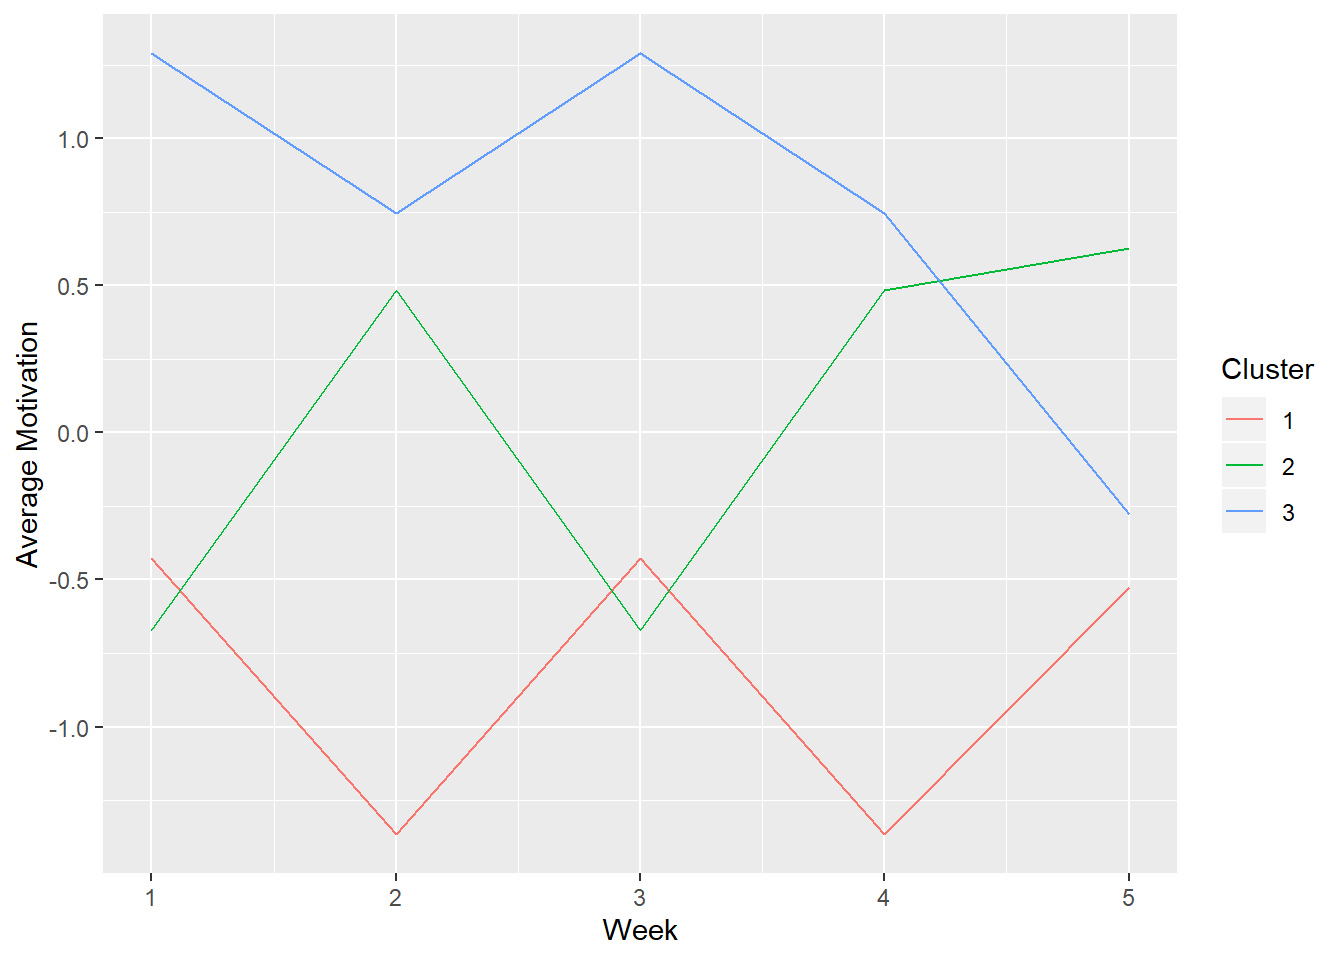
\includegraphics{Assignment-3_files/figure-latex/unnamed-chunk-10-1.pdf}

What patterns do you see in the plot?

We saw two clusters of the average motivation. One is generally higher
and another is lower.

It would be useful to determine how many people are in each cluster. We
can do this easily with dplyr.

\begin{Shaded}
\begin{Highlighting}[]
\NormalTok{K7 <-}\StringTok{ }\NormalTok{dplyr}\OperatorTok{::}\KeywordTok{count}\NormalTok{(K4, cluster)}
\NormalTok{K7}
\end{Highlighting}
\end{Shaded}

\begin{verbatim}
## # A tibble: 2 x 2
##   cluster     n
##     <int> <int>
## 1       1     8
## 2       2    15
\end{verbatim}

Look at the number of people in each cluster, now repeat this process
for 3 rather than 2 clusters. Which cluster grouping do you think is
more informative? Write your answer below:

\begin{Shaded}
\begin{Highlighting}[]
\NormalTok{fit <-}\StringTok{ }\KeywordTok{kmeans}\NormalTok{(K3,}\DecValTok{3}\NormalTok{)}
\NormalTok{fit}
\end{Highlighting}
\end{Shaded}

\begin{verbatim}
## K-means clustering with 3 clusters of sizes 7, 9, 7
## 
## Cluster means:
##   motivation1 motivation2 motivation3 motivation4 motivation5
## 1  -0.4261330  -1.3666757  -0.4261330  -1.3666757  -0.5258485
## 2  -0.6711594   0.4823561  -0.6711594   0.4823561   0.6260101
## 3   1.2890523   0.7465036   1.2890523   0.7465036  -0.2790216
## 
## Clustering vector:
##  1  3  7 10 12 14 15 17 18 19 20 22 25 26 27 28 29 30 31 32 33 34 35 
##  3  2  3  3  1  3  1  1  1  1  3  3  1  2  2  2  2  2  2  2  2  1  3 
## 
## Within cluster sum of squares by cluster:
## [1] 11.013691  2.985251 17.940856
##  (between_SS / total_SS =  71.0 %)
## 
## Available components:
## 
## [1] "cluster"      "centers"      "totss"        "withinss"    
## [5] "tot.withinss" "betweenss"    "size"         "iter"        
## [9] "ifault"
\end{verbatim}

\begin{Shaded}
\begin{Highlighting}[]
\NormalTok{K4<-}\KeywordTok{data.frame}\NormalTok{(K3,fit}\OperatorTok{$}\NormalTok{cluster)}
\NormalTok{K4}
\end{Highlighting}
\end{Shaded}

\begin{verbatim}
##    motivation1 motivation2 motivation3 motivation4 motivation5 fit.cluster
## 1    1.0440258   0.4823561   1.0440258   0.4823561  -0.5258485           3
## 3   -0.6711594   0.4823561  -0.6711594   0.4823561  -0.5258485           2
## 7    1.0440258   0.4823561   1.0440258   0.4823561  -0.5258485           3
## 10   1.0440258   0.4823561   1.0440258   0.4823561  -0.5258485           3
## 12   1.0440258  -1.3666757   1.0440258  -1.3666757  -0.5258485           1
## 14   1.0440258   2.3313880   1.0440258   2.3313880  -1.3897424           3
## 15  -0.6711594  -1.3666757  -0.6711594  -1.3666757   1.2019394           1
## 17  -0.6711594  -1.3666757  -0.6711594  -1.3666757   0.3380454           1
## 18  -0.6711594  -1.3666757  -0.6711594  -1.3666757  -1.3897424           1
## 19  -0.6711594  -1.3666757  -0.6711594  -1.3666757  -1.3897424           1
## 20   2.7592111   0.4823561   2.7592111   0.4823561  -0.5258485           3
## 22   1.0440258   0.4823561   1.0440258   0.4823561   2.0658333           3
## 25  -0.6711594  -1.3666757  -0.6711594  -1.3666757  -0.5258485           1
## 26  -0.6711594   0.4823561  -0.6711594   0.4823561   1.2019394           2
## 27  -0.6711594   0.4823561  -0.6711594   0.4823561   0.3380454           2
## 28  -0.6711594   0.4823561  -0.6711594   0.4823561   1.2019394           2
## 29  -0.6711594   0.4823561  -0.6711594   0.4823561   0.3380454           2
## 30  -0.6711594   0.4823561  -0.6711594   0.4823561   1.2019394           2
## 31  -0.6711594   0.4823561  -0.6711594   0.4823561   0.3380454           2
## 32  -0.6711594   0.4823561  -0.6711594   0.4823561   1.2019394           2
## 33  -0.6711594   0.4823561  -0.6711594   0.4823561   0.3380454           2
## 34  -0.6711594  -1.3666757  -0.6711594  -1.3666757  -1.3897424           1
## 35   1.0440258   0.4823561   1.0440258   0.4823561  -0.5258485           3
\end{verbatim}

\begin{Shaded}
\begin{Highlighting}[]
\KeywordTok{names}\NormalTok{(K4)[}\KeywordTok{names}\NormalTok{(K4) }\OperatorTok{==}\StringTok{ "fit.cluster"}\NormalTok{] <-}\StringTok{ "cluster"}
\KeywordTok{names}\NormalTok{(K4)[}\KeywordTok{names}\NormalTok{(K4) }\OperatorTok{==}\StringTok{ "motivation1"}\NormalTok{] <-}\StringTok{ "1"}
\KeywordTok{names}\NormalTok{(K4)[}\KeywordTok{names}\NormalTok{(K4) }\OperatorTok{==}\StringTok{ "motivation2"}\NormalTok{] <-}\StringTok{ "2"}
\KeywordTok{names}\NormalTok{(K4)[}\KeywordTok{names}\NormalTok{(K4) }\OperatorTok{==}\StringTok{ "motivation3"}\NormalTok{] <-}\StringTok{ "3"}
\KeywordTok{names}\NormalTok{(K4)[}\KeywordTok{names}\NormalTok{(K4) }\OperatorTok{==}\StringTok{ "motivation4"}\NormalTok{] <-}\StringTok{ "4"}
\KeywordTok{names}\NormalTok{(K4)[}\KeywordTok{names}\NormalTok{(K4) }\OperatorTok{==}\StringTok{ "motivation5"}\NormalTok{] <-}\StringTok{ "5"}
\NormalTok{K4}
\end{Highlighting}
\end{Shaded}

\begin{verbatim}
##             1          2          3          4          5 cluster
## 1   1.0440258  0.4823561  1.0440258  0.4823561 -0.5258485       3
## 3  -0.6711594  0.4823561 -0.6711594  0.4823561 -0.5258485       2
## 7   1.0440258  0.4823561  1.0440258  0.4823561 -0.5258485       3
## 10  1.0440258  0.4823561  1.0440258  0.4823561 -0.5258485       3
## 12  1.0440258 -1.3666757  1.0440258 -1.3666757 -0.5258485       1
## 14  1.0440258  2.3313880  1.0440258  2.3313880 -1.3897424       3
## 15 -0.6711594 -1.3666757 -0.6711594 -1.3666757  1.2019394       1
## 17 -0.6711594 -1.3666757 -0.6711594 -1.3666757  0.3380454       1
## 18 -0.6711594 -1.3666757 -0.6711594 -1.3666757 -1.3897424       1
## 19 -0.6711594 -1.3666757 -0.6711594 -1.3666757 -1.3897424       1
## 20  2.7592111  0.4823561  2.7592111  0.4823561 -0.5258485       3
## 22  1.0440258  0.4823561  1.0440258  0.4823561  2.0658333       3
## 25 -0.6711594 -1.3666757 -0.6711594 -1.3666757 -0.5258485       1
## 26 -0.6711594  0.4823561 -0.6711594  0.4823561  1.2019394       2
## 27 -0.6711594  0.4823561 -0.6711594  0.4823561  0.3380454       2
## 28 -0.6711594  0.4823561 -0.6711594  0.4823561  1.2019394       2
## 29 -0.6711594  0.4823561 -0.6711594  0.4823561  0.3380454       2
## 30 -0.6711594  0.4823561 -0.6711594  0.4823561  1.2019394       2
## 31 -0.6711594  0.4823561 -0.6711594  0.4823561  0.3380454       2
## 32 -0.6711594  0.4823561 -0.6711594  0.4823561  1.2019394       2
## 33 -0.6711594  0.4823561 -0.6711594  0.4823561  0.3380454       2
## 34 -0.6711594 -1.3666757 -0.6711594 -1.3666757 -1.3897424       1
## 35  1.0440258  0.4823561  1.0440258  0.4823561 -0.5258485       3
\end{verbatim}

\begin{Shaded}
\begin{Highlighting}[]
\NormalTok{K5 <-}\StringTok{ }\NormalTok{(}\KeywordTok{gather}\NormalTok{(K4, }\StringTok{"week"}\NormalTok{,}\StringTok{"motivation"}\NormalTok{, }\DecValTok{1}\OperatorTok{:}\DecValTok{5}\NormalTok{))}
\NormalTok{K5[, }\StringTok{'week'}\NormalTok{] <-}\StringTok{ }\KeywordTok{as.factor}\NormalTok{(K5[, }\StringTok{'week'}\NormalTok{])}

\NormalTok{K5<-}\KeywordTok{data.frame}\NormalTok{(K5)}
\NormalTok{K5}
\end{Highlighting}
\end{Shaded}

\begin{verbatim}
##     cluster week motivation
## 1         3    1  1.0440258
## 2         2    1 -0.6711594
## 3         3    1  1.0440258
## 4         3    1  1.0440258
## 5         1    1  1.0440258
## 6         3    1  1.0440258
## 7         1    1 -0.6711594
## 8         1    1 -0.6711594
## 9         1    1 -0.6711594
## 10        1    1 -0.6711594
## 11        3    1  2.7592111
## 12        3    1  1.0440258
## 13        1    1 -0.6711594
## 14        2    1 -0.6711594
## 15        2    1 -0.6711594
## 16        2    1 -0.6711594
## 17        2    1 -0.6711594
## 18        2    1 -0.6711594
## 19        2    1 -0.6711594
## 20        2    1 -0.6711594
## 21        2    1 -0.6711594
## 22        1    1 -0.6711594
## 23        3    1  1.0440258
## 24        3    2  0.4823561
## 25        2    2  0.4823561
## 26        3    2  0.4823561
## 27        3    2  0.4823561
## 28        1    2 -1.3666757
## 29        3    2  2.3313880
## 30        1    2 -1.3666757
## 31        1    2 -1.3666757
## 32        1    2 -1.3666757
## 33        1    2 -1.3666757
## 34        3    2  0.4823561
## 35        3    2  0.4823561
## 36        1    2 -1.3666757
## 37        2    2  0.4823561
## 38        2    2  0.4823561
## 39        2    2  0.4823561
## 40        2    2  0.4823561
## 41        2    2  0.4823561
## 42        2    2  0.4823561
## 43        2    2  0.4823561
## 44        2    2  0.4823561
## 45        1    2 -1.3666757
## 46        3    2  0.4823561
## 47        3    3  1.0440258
## 48        2    3 -0.6711594
## 49        3    3  1.0440258
## 50        3    3  1.0440258
## 51        1    3  1.0440258
## 52        3    3  1.0440258
## 53        1    3 -0.6711594
## 54        1    3 -0.6711594
## 55        1    3 -0.6711594
## 56        1    3 -0.6711594
## 57        3    3  2.7592111
## 58        3    3  1.0440258
## 59        1    3 -0.6711594
## 60        2    3 -0.6711594
## 61        2    3 -0.6711594
## 62        2    3 -0.6711594
## 63        2    3 -0.6711594
## 64        2    3 -0.6711594
## 65        2    3 -0.6711594
## 66        2    3 -0.6711594
## 67        2    3 -0.6711594
## 68        1    3 -0.6711594
## 69        3    3  1.0440258
## 70        3    4  0.4823561
## 71        2    4  0.4823561
## 72        3    4  0.4823561
## 73        3    4  0.4823561
## 74        1    4 -1.3666757
## 75        3    4  2.3313880
## 76        1    4 -1.3666757
## 77        1    4 -1.3666757
## 78        1    4 -1.3666757
## 79        1    4 -1.3666757
## 80        3    4  0.4823561
## 81        3    4  0.4823561
## 82        1    4 -1.3666757
## 83        2    4  0.4823561
## 84        2    4  0.4823561
## 85        2    4  0.4823561
## 86        2    4  0.4823561
## 87        2    4  0.4823561
## 88        2    4  0.4823561
## 89        2    4  0.4823561
## 90        2    4  0.4823561
## 91        1    4 -1.3666757
## 92        3    4  0.4823561
## 93        3    5 -0.5258485
## 94        2    5 -0.5258485
## 95        3    5 -0.5258485
## 96        3    5 -0.5258485
## 97        1    5 -0.5258485
## 98        3    5 -1.3897424
## 99        1    5  1.2019394
## 100       1    5  0.3380454
## 101       1    5 -1.3897424
## 102       1    5 -1.3897424
## 103       3    5 -0.5258485
## 104       3    5  2.0658333
## 105       1    5 -0.5258485
## 106       2    5  1.2019394
## 107       2    5  0.3380454
## 108       2    5  1.2019394
## 109       2    5  0.3380454
## 110       2    5  1.2019394
## 111       2    5  0.3380454
## 112       2    5  1.2019394
## 113       2    5  0.3380454
## 114       1    5 -1.3897424
## 115       3    5 -0.5258485
\end{verbatim}

\begin{Shaded}
\begin{Highlighting}[]
\NormalTok{K6 <-}\StringTok{ }\NormalTok{K5 }\OperatorTok\StringTok{ }\KeywordTok{group_by}\NormalTok{(week,cluster)}
\NormalTok{K6<-}\StringTok{ }\KeywordTok{summarise}\NormalTok{(K6,}\DataTypeTok{cluster_mean=} \KeywordTok{mean}\NormalTok{(motivation))}
\NormalTok{K6}
\end{Highlighting}
\end{Shaded}

\begin{verbatim}
## # A tibble: 15 x 3
## # Groups:   week [5]
##    week  cluster cluster_mean
##    <fct>   <int>        <dbl>
##  1 1           1       -0.426
##  2 1           2       -0.671
##  3 1           3        1.29 
##  4 2           1       -1.37 
##  5 2           2        0.482
##  6 2           3        0.747
##  7 3           1       -0.426
##  8 3           2       -0.671
##  9 3           3        1.29 
## 10 4           1       -1.37 
## 11 4           2        0.482
## 12 4           3        0.747
## 13 5           1       -0.526
## 14 5           2        0.626
## 15 5           3       -0.279
\end{verbatim}

\begin{Shaded}
\begin{Highlighting}[]
\NormalTok{K6}\OperatorTok{$}\NormalTok{week  <-}\StringTok{ }\KeywordTok{as_factor}\NormalTok{(K6}\OperatorTok{$}\NormalTok{week)}

\NormalTok{K6}\OperatorTok{$}\NormalTok{cluster <-}\StringTok{ }\KeywordTok{as.factor}\NormalTok{(K6}\OperatorTok{$}\NormalTok{cluster)}
\NormalTok{K6}
\end{Highlighting}
\end{Shaded}

\begin{verbatim}
## # A tibble: 15 x 3
## # Groups:   week [5]
##    week  cluster cluster_mean
##    <fct> <fct>          <dbl>
##  1 1     1             -0.426
##  2 1     2             -0.671
##  3 1     3              1.29 
##  4 2     1             -1.37 
##  5 2     2              0.482
##  6 2     3              0.747
##  7 3     1             -0.426
##  8 3     2             -0.671
##  9 3     3              1.29 
## 10 4     1             -1.37 
## 11 4     2              0.482
## 12 4     3              0.747
## 13 5     1             -0.526
## 14 5     2              0.626
## 15 5     3             -0.279
\end{verbatim}

\begin{Shaded}
\begin{Highlighting}[]
\NormalTok{plot5 <-}\StringTok{ }\KeywordTok{ggplot}\NormalTok{(K6, }\KeywordTok{aes}\NormalTok{(week, cluster_mean, }\DataTypeTok{group =}\NormalTok{ cluster)) }\OperatorTok{+}
\StringTok{         }\KeywordTok{geom_point}\NormalTok{() }\OperatorTok{+}
\StringTok{         }\KeywordTok{geom_line}\NormalTok{() }\OperatorTok{+}
\StringTok{         }\KeywordTok{labs}\NormalTok{(}\DataTypeTok{x =} \StringTok{"Week"}\NormalTok{, }\DataTypeTok{y =} \StringTok{"Average Motivation"}\NormalTok{, }
              \DataTypeTok{title =} \StringTok{"Clustering plot"}\NormalTok{)}
\NormalTok{plot5}
\end{Highlighting}
\end{Shaded}

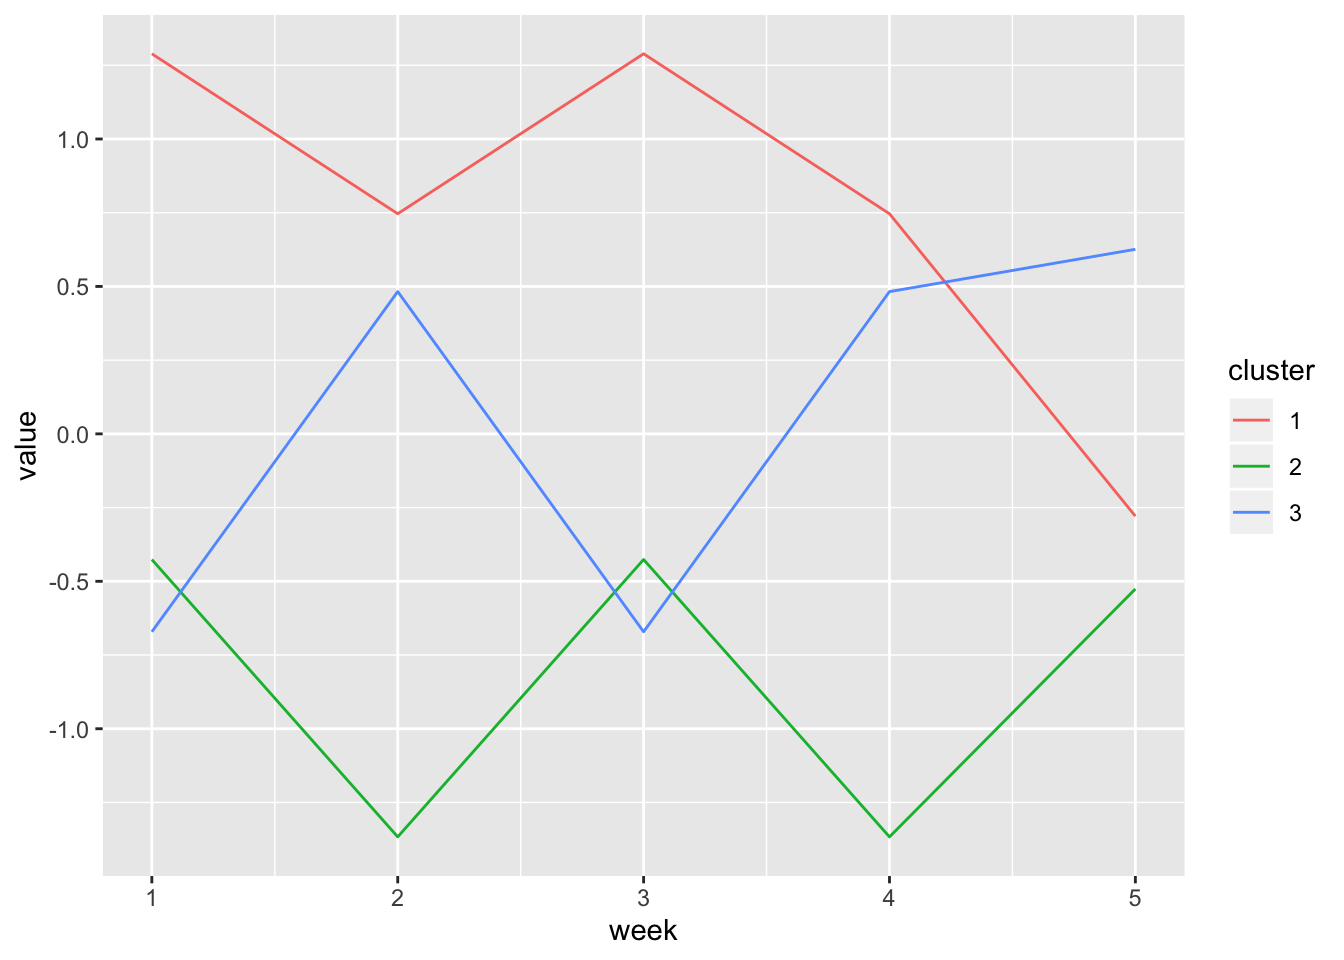
\includegraphics{Assignment-3_files/figure-latex/unnamed-chunk-12-1.pdf}

\begin{Shaded}
\begin{Highlighting}[]
\NormalTok{K7 <-}\StringTok{ }\NormalTok{dplyr}\OperatorTok{::}\KeywordTok{count}\NormalTok{(K4, cluster)}
\NormalTok{K7}
\end{Highlighting}
\end{Shaded}

\begin{verbatim}
## # A tibble: 3 x 2
##   cluster     n
##     <int> <int>
## 1       1     7
## 2       2     9
## 3       3     7
\end{verbatim}

\#\#Part II

Using the data collected for Assignment 2 (which classes students were
in), cluster the students, then redraw the graph of the class but color
the students according the cluster they are in.

\begin{Shaded}
\begin{Highlighting}[]
\NormalTok{raw_data <-}\StringTok{ }\KeywordTok{read.csv}\NormalTok{(}\StringTok{"~/Desktop/2019fall/core methods in edm/assignment2/assignment 1015/hudk4050-classes.csv"}\NormalTok{)}
\CommentTok{#select useful columns}
\KeywordTok{install.packages}\NormalTok{((}\StringTok{"tidyverse"}\NormalTok{),}\DataTypeTok{repos =} \StringTok{"http://cran.us.r-project.org"}\NormalTok{)}
\end{Highlighting}
\end{Shaded}

\begin{verbatim}
## 
## The downloaded binary packages are in
##  /var/folders/7n/3w87168x3kv3dj0nskjj52r80000gp/T//RtmpPI5jQH/downloaded_packages
\end{verbatim}

\begin{Shaded}
\begin{Highlighting}[]
\KeywordTok{install.packages}\NormalTok{((}\StringTok{"tidyr"}\NormalTok{),}\DataTypeTok{repos =} \StringTok{"http://cran.us.r-project.org"}\NormalTok{)}
\end{Highlighting}
\end{Shaded}

\begin{verbatim}
## 
## The downloaded binary packages are in
##  /var/folders/7n/3w87168x3kv3dj0nskjj52r80000gp/T//RtmpPI5jQH/downloaded_packages
\end{verbatim}

\begin{Shaded}
\begin{Highlighting}[]
\KeywordTok{library}\NormalTok{(tidyr)}
\KeywordTok{install.packages}\NormalTok{((}\StringTok{"dplyr"}\NormalTok{),}\DataTypeTok{repos =} \StringTok{"http://cran.us.r-project.org"}\NormalTok{)}
\end{Highlighting}
\end{Shaded}

\begin{verbatim}
## 
## The downloaded binary packages are in
##  /var/folders/7n/3w87168x3kv3dj0nskjj52r80000gp/T//RtmpPI5jQH/downloaded_packages
\end{verbatim}

\begin{Shaded}
\begin{Highlighting}[]
\NormalTok{data_new<-}\KeywordTok{unite}\NormalTok{(raw_data, Name, }\StringTok{"First.Name"}\NormalTok{,}\StringTok{"Last.Name"}\NormalTok{, }\DataTypeTok{sep =} \StringTok{" "}\NormalTok{)}
\NormalTok{data_new}
\end{Highlighting}
\end{Shaded}

\begin{verbatim}
##       Start.Date      End.Date Response.Type    IP.Address Progress
## 1  10/3/19 15:14 10/3/19 15:15    IP Address 160.39.69.129      100
## 2  10/3/19 15:14 10/3/19 15:15    IP Address  160.39.69.28      100
## 3  10/3/19 15:14 10/3/19 15:16    IP Address 160.39.69.129      100
## 4  10/3/19 15:14 10/3/19 15:16    IP Address 160.39.69.129      100
## 5  10/3/19 15:14 10/3/19 15:16    IP Address 160.39.69.129      100
## 6  10/3/19 15:14 10/3/19 15:16    IP Address 160.39.69.129      100
## 7  10/3/19 15:15 10/3/19 15:16    IP Address 160.39.69.129      100
## 8  10/3/19 15:14 10/3/19 15:16    IP Address 160.39.69.129      100
## 9  10/3/19 15:14 10/3/19 15:16    IP Address  160.39.69.28      100
## 10 10/3/19 15:15 10/3/19 15:16    IP Address 160.39.69.129      100
## 11 10/3/19 15:14 10/3/19 15:16    IP Address 160.39.69.129      100
## 12 10/3/19 15:14 10/3/19 15:16    IP Address 160.39.69.129      100
## 13 10/3/19 15:14 10/3/19 15:16    IP Address  160.39.69.28      100
## 14 10/3/19 15:14 10/3/19 15:16    IP Address 160.39.69.129      100
## 15 10/3/19 15:15 10/3/19 15:16    IP Address 160.39.69.129      100
## 16 10/3/19 15:14 10/3/19 15:17    IP Address 160.39.69.129      100
## 17 10/3/19 15:14 10/3/19 15:17    IP Address 160.39.69.129      100
## 18 10/3/19 15:14 10/3/19 15:17    IP Address 160.39.69.129      100
## 19 10/3/19 15:14 10/3/19 15:17    IP Address 160.39.69.129      100
## 20 10/3/19 15:14 10/3/19 15:17    IP Address 160.39.69.129      100
## 21 10/3/19 15:14 10/3/19 15:17    IP Address 160.39.69.129      100
## 22 10/3/19 15:15 10/3/19 15:17    IP Address 160.39.69.129      100
## 23 10/3/19 15:15 10/3/19 15:17    IP Address 160.39.69.129      100
## 24 10/3/19 15:14 10/3/19 15:17    IP Address  160.39.69.28      100
## 25 10/3/19 15:14 10/3/19 15:17    IP Address 160.39.69.129      100
## 26 10/3/19 15:14 10/3/19 15:18    IP Address 160.39.69.129      100
## 27 10/3/19 15:15 10/3/19 15:18    IP Address 160.39.69.129      100
## 28 10/3/19 15:14 10/3/19 15:18    IP Address 160.39.69.129      100
## 29 10/3/19 15:14 10/3/19 15:18    IP Address  160.39.69.28      100
## 30 10/3/19 15:16 10/3/19 15:18    IP Address 160.39.69.129      100
## 31 10/3/19 15:14 10/3/19 15:18    IP Address 160.39.69.129      100
## 32 10/3/19 15:14 10/3/19 15:18    IP Address 160.39.69.129      100
## 33 10/3/19 15:15 10/3/19 15:18    IP Address  160.39.69.28      100
## 34 10/3/19 15:17 10/3/19 15:18    IP Address 160.39.69.129      100
## 35 10/3/19 15:17 10/3/19 15:18    IP Address  160.39.69.28      100
## 36 10/3/19 15:17 10/3/19 15:18    IP Address  160.39.69.28      100
## 37 10/3/19 15:16 10/3/19 15:18    IP Address 160.39.69.129      100
## 38 10/3/19 15:15 10/3/19 15:18    IP Address 160.39.69.129      100
## 39 10/3/19 15:14 10/3/19 15:18    IP Address 160.39.69.129      100
## 40 10/3/19 15:14 10/3/19 15:18    IP Address 160.39.69.129      100
## 41 10/3/19 15:14 10/3/19 15:18    IP Address 160.39.69.129      100
## 42 10/3/19 15:14 10/3/19 15:18    IP Address 160.39.69.129      100
## 43 10/3/19 15:14 10/3/19 15:18    IP Address  160.39.69.28      100
## 44 10/3/19 15:16 10/3/19 15:18    IP Address  160.39.69.28      100
## 45 10/3/19 15:14 10/3/19 15:19    IP Address 160.39.69.129      100
## 46 10/3/19 15:14 10/3/19 15:19    IP Address 160.39.69.129      100
## 47 10/3/19 15:15 10/3/19 15:19    IP Address 160.39.69.129      100
## 48 10/3/19 15:14 10/3/19 15:19    IP Address 160.39.69.129      100
## 49 10/3/19 15:16 10/3/19 15:21    IP Address  160.39.69.28      100
## 50 10/3/19 15:19 10/3/19 15:27    IP Address 160.39.69.129      100
## 51 10/3/19 15:23 10/3/19 15:28    IP Address 172.58.235.63      100
## 52 10/3/19 15:15 10/3/19 15:44    IP Address  160.39.69.28      100
## 53 10/3/19 15:14 10/3/19 15:47    IP Address 160.39.69.129      100
##    Duration..in.seconds. Finished Recorded.Date       Response.ID
## 1                     87     TRUE 10/3/19 15:15 R_27dJLX5hbdxjUoR
## 2                     72     TRUE 10/3/19 15:15 R_5iMeogh9eblmKml
## 3                     92     TRUE 10/3/19 15:16 R_2PBDZUj91ZLieEG
## 4                     89     TRUE 10/3/19 15:16 R_TcSbqrLAvFdIPqV
## 5                     95     TRUE 10/3/19 15:16 R_3HC97LFgU5DZru2
## 6                     80     TRUE 10/3/19 15:16 R_1rBtDP9kpwXmQ79
## 7                     66     TRUE 10/3/19 15:16 R_1mqHZTquhCweI7n
## 8                    105     TRUE 10/3/19 15:16 R_2DOmRnikBCqIq6e
## 9                    122     TRUE 10/3/19 15:16 R_1QmRu26LD6MGEze
## 10                    62     TRUE 10/3/19 15:16 R_YX2DnCiQTzgbMn7
## 11                   144     TRUE 10/3/19 15:16 R_2c165wrzVdhz3Dc
## 12                   126     TRUE 10/3/19 15:16 R_urJtBRAXy6FQeVH
## 13                   159     TRUE 10/3/19 15:16 R_2uNU9ZbZpepw6Rb
## 14                   118     TRUE 10/3/19 15:16 R_6Xw4usZOXrDvC3T
## 15                    70     TRUE 10/3/19 15:16 R_3fUDfoBX0hoCL6J
## 16                   151     TRUE 10/3/19 15:17 R_3MijAmcOkAyJrfP
## 17                   163     TRUE 10/3/19 15:17 R_2E9VCHYM93KuxOy
## 18                   186     TRUE 10/3/19 15:17 R_1NF8yJ5Ok9lkQm7
## 19                   158     TRUE 10/3/19 15:17 R_2S1UmcQ2jVajs8e
## 20                   155     TRUE 10/3/19 15:17 R_ebSole9AhZKmCZP
## 21                   162     TRUE 10/3/19 15:17 R_1Ntu2tkMN6mOzHa
## 22                   142     TRUE 10/3/19 15:17 R_2s6j78wCDgaep1V
## 23                   158     TRUE 10/3/19 15:17 R_2zdW6dJE4rXbquD
## 24                   166     TRUE 10/3/19 15:17 R_1OI85NgX9RJufcQ
## 25                   174     TRUE 10/3/19 15:17 R_1DPckCcNUFqD7o7
## 26                   208     TRUE 10/3/19 15:18 R_sv4ED1kwW93m5CV
## 27                   175     TRUE 10/3/19 15:18 R_1hYdq1FHyZ0iFTT
## 28                   209     TRUE 10/3/19 15:18 R_27NK13IpZP2AADM
## 29                   217     TRUE 10/3/19 15:18 R_3ndCM7SHRXHPGsK
## 30                    85     TRUE 10/3/19 15:18 R_3EQ2EXsAeTyQFNW
## 31                   211     TRUE 10/3/19 15:18 R_2yjXiMjdk6hXO9n
## 32                   217     TRUE 10/3/19 15:18 R_2fk9oC8JUdNdqFn
## 33                   163     TRUE 10/3/19 15:18 R_33lsAhghE4hAC1u
## 34                    52     TRUE 10/3/19 15:18 R_2Tpj0MpsyzEpQsy
## 35                    74     TRUE 10/3/19 15:18 R_1OIuLXOOqMdfCeV
## 36                    54     TRUE 10/3/19 15:18 R_31RTIRsgjZW7rw7
## 37                   134     TRUE 10/3/19 15:18 R_3MsVhg9ACOUgsR3
## 38                   184     TRUE 10/3/19 15:18 R_3Jxb82Gzl9u2H1L
## 39                   248     TRUE 10/3/19 15:18 R_9SIx7QbtsTlismZ
## 40                   259     TRUE 10/3/19 15:18 R_30qTnVlRvPUGWGI
## 41                   232     TRUE 10/3/19 15:18 R_3CrE39NRq8M1tVD
## 42                   249     TRUE 10/3/19 15:18 R_3ezDHe5GFBWreTI
## 43                   264     TRUE 10/3/19 15:18 R_2aIxBdruL2dOEMd
## 44                   171     TRUE 10/3/19 15:18 R_2SpYZYRtS9bTGCU
## 45                   268     TRUE 10/3/19 15:19 R_1Q0l7L2OctsFxVC
## 46                   304     TRUE 10/3/19 15:19 R_3GozoBcPMx5Gbsc
## 47                   222     TRUE 10/3/19 15:19 R_3exf52H2nv2ns8z
## 48                   312     TRUE 10/3/19 15:19 R_3nCRn7ALL9Wcyx6
## 49                   307     TRUE 10/3/19 15:21 R_214DiGxiPYEJQO3
## 50                   474     TRUE 10/3/19 15:27 R_V21R9DlAPZBSfux
## 51                   288     TRUE 10/3/19 15:28 R_1ODG5LnfvKpBZIu
## 52                  1711     TRUE 10/3/19 15:44 R_1pLlUcOHWHjy6C1
## 53                  1977     TRUE 10/3/19 15:47 R_2B35cGkqBuD0Ov5
##    Recipient.Last.Name Recipient.First.Name Recipient.Email
## 1                   NA                   NA              NA
## 2                   NA                   NA              NA
## 3                   NA                   NA              NA
## 4                   NA                   NA              NA
## 5                   NA                   NA              NA
## 6                   NA                   NA              NA
## 7                   NA                   NA              NA
## 8                   NA                   NA              NA
## 9                   NA                   NA              NA
## 10                  NA                   NA              NA
## 11                  NA                   NA              NA
## 12                  NA                   NA              NA
## 13                  NA                   NA              NA
## 14                  NA                   NA              NA
## 15                  NA                   NA              NA
## 16                  NA                   NA              NA
## 17                  NA                   NA              NA
## 18                  NA                   NA              NA
## 19                  NA                   NA              NA
## 20                  NA                   NA              NA
## 21                  NA                   NA              NA
## 22                  NA                   NA              NA
## 23                  NA                   NA              NA
## 24                  NA                   NA              NA
## 25                  NA                   NA              NA
## 26                  NA                   NA              NA
## 27                  NA                   NA              NA
## 28                  NA                   NA              NA
## 29                  NA                   NA              NA
## 30                  NA                   NA              NA
## 31                  NA                   NA              NA
## 32                  NA                   NA              NA
## 33                  NA                   NA              NA
## 34                  NA                   NA              NA
## 35                  NA                   NA              NA
## 36                  NA                   NA              NA
## 37                  NA                   NA              NA
## 38                  NA                   NA              NA
## 39                  NA                   NA              NA
## 40                  NA                   NA              NA
## 41                  NA                   NA              NA
## 42                  NA                   NA              NA
## 43                  NA                   NA              NA
## 44                  NA                   NA              NA
## 45                  NA                   NA              NA
## 46                  NA                   NA              NA
## 47                  NA                   NA              NA
## 48                  NA                   NA              NA
## 49                  NA                   NA              NA
## 50                  NA                   NA              NA
## 51                  NA                   NA              NA
## 52                  NA                   NA              NA
## 53                  NA                   NA              NA
##    External.Data.Reference Location.Latitude Location.Longitude
## 1                       NA           40.8000           -73.9763
## 2                       NA           40.8000           -73.9763
## 3                       NA           40.8000           -73.9763
## 4                       NA           40.8000           -73.9763
## 5                       NA           40.8000           -73.9763
## 6                       NA           40.8000           -73.9763
## 7                       NA           40.8000           -73.9763
## 8                       NA           40.8000           -73.9763
## 9                       NA           40.8000           -73.9763
## 10                      NA           40.8000           -73.9763
## 11                      NA           40.8000           -73.9763
## 12                      NA           40.8000           -73.9763
## 13                      NA           40.8000           -73.9763
## 14                      NA           40.8000           -73.9763
## 15                      NA           40.8000           -73.9763
## 16                      NA           40.8000           -73.9763
## 17                      NA           40.8000           -73.9763
## 18                      NA           40.8000           -73.9763
## 19                      NA           40.8000           -73.9763
## 20                      NA           40.8000           -73.9763
## 21                      NA           40.8000           -73.9763
## 22                      NA           40.8000           -73.9763
## 23                      NA           40.8000           -73.9763
## 24                      NA           40.8000           -73.9763
## 25                      NA           40.8000           -73.9763
## 26                      NA           40.8000           -73.9763
## 27                      NA           40.8000           -73.9763
## 28                      NA           40.8000           -73.9763
## 29                      NA           40.8000           -73.9763
## 30                      NA           40.8000           -73.9763
## 31                      NA           40.8000           -73.9763
## 32                      NA           40.8000           -73.9763
## 33                      NA           40.8000           -73.9763
## 34                      NA           40.8000           -73.9763
## 35                      NA           40.8000           -73.9763
## 36                      NA           40.8000           -73.9763
## 37                      NA           40.8000           -73.9763
## 38                      NA           40.8000           -73.9763
## 39                      NA           40.8000           -73.9763
## 40                      NA           40.8000           -73.9763
## 41                      NA           40.8000           -73.9763
## 42                      NA           40.8000           -73.9763
## 43                      NA           40.8000           -73.9763
## 44                      NA           40.8000           -73.9763
## 45                      NA           40.8000           -73.9763
## 46                      NA           40.8000           -73.9763
## 47                      NA           40.8000           -73.9763
## 48                      NA           40.8000           -73.9763
## 49                      NA           40.8000           -73.9763
## 50                      NA           40.8000           -73.9763
## 51                      NA           40.7415           -74.2330
## 52                      NA           40.8000           -73.9763
## 53                      NA           40.8000           -73.9763
##    Distribution.Channel User.Language              Name
## 1             anonymous            EN      Artemas Wang
## 2             anonymous            EN         Yawei Zhu
## 3             anonymous            EN        Ningyao Xu
## 4             anonymous            EN        Qiyang Lin
## 5             anonymous            EN    Bernell Downer
## 6             anonymous            EN        Ruiqi Wang
## 7             anonymous            EN Leonardo Restrepo
## 8             anonymous            EN    Zhaozhuo Zheng
## 9             anonymous            EN    Jiancong  Shen
## 10            anonymous            EN         ZIFAN CAO
## 11            anonymous            EN    Allison Teevan
## 12            anonymous            EN          Yiwen Ma
## 13            anonymous            EN        Beibei Cao
## 14            anonymous            EN         yixiao li
## 15            anonymous            EN        xinyi zhou
## 16            anonymous            EN      Jingru Zhang
## 17            anonymous            EN        Ziyuan Guo
## 18            anonymous            EN       Timothy Lee
## 19            anonymous            EN           XI YANG
## 20            anonymous            EN        Chenyu Yan
## 21            anonymous            EN          Yiyi Xie
## 22            anonymous            EN            Di Mao
## 23            anonymous            EN          Han Wang
## 24            anonymous            EN      Xiaowen Chen
## 25            anonymous            EN         Anqi Duan
## 26            anonymous            EN           Ling Ai
## 27            anonymous            EN          Yiwei Qi
## 28            anonymous            EN        jiahao guo
## 29            anonymous            EN     LINGLING MIAO
## 30            anonymous            EN      Shijie  Shao
## 31            anonymous            EN       Yujun Zhang
## 32            anonymous            EN    chaoxiong chen
## 33            anonymous            EN        Lintong Li
## 34            anonymous            EN         ZIMO CHEN
## 35            anonymous            EN            HAN GE
## 36            anonymous            EN   Alysandra Zhang
## 37            anonymous            EN        Yixuan Zhu
## 38            anonymous            EN      XUDIAN ZHANG
## 39            anonymous            EN           YAQI LU
## 40            anonymous            EN Christine Odenath
## 41            anonymous            EN      David Pearce
## 42            anonymous            EN      Chengxuan Hu
## 43            anonymous            EN   Zhongyuan Zhang
## 44            anonymous            EN      Maho Hayashi
## 45            anonymous            EN       Minruo Wang
## 46            anonymous            EN          Jie Chen
## 47            anonymous            EN   INDIRA BATAYEVA
## 48            anonymous            EN  Eudora Xinyi Niu
## 49            anonymous            EN      Joellyn Heng
## 50            anonymous            EN         Yigao Liu
## 51            anonymous            EN      Wanruo Zhang
## 52            anonymous            EN       Suwon  Jung
## 53            anonymous            EN          Luyi Dai
##    UNI..the.two.letters.followed.by.four.numbers.that.make.up.your.email.address..eg.kh4513.
## 1                                                                                    adw2184
## 2                                                                                     yz3413
## 3                                                                                     nx2150
## 4                                                                                     ql2360
## 5                                                                                    bkd2115
## 6                                                                                     RW2796
## 7                                                                                     lr2956
## 8                                                                                     zz2726
## 9                                                                                     js5498
## 10                                                                                    ZC2323
## 11                                                                                   art2172
## 12                                                                                    ym2775
## 13                                                                                    bc2824
## 14                                                                                    yl4284
## 15                                                                                    XZ2910
## 16                                                                                    jz3101
## 17                                                                                    zg2338
## 18                                                                                   xql2001
## 19                                                                                    XY2418
## 20                                                                                    cy2535
## 21                                                                                    yx2531
## 22                                                                                    dm3487
## 23                                                                                    hw2663
## 24                                                                                    xc2496
## 25                                                                                    ad3671
## 26                                                                                    la2738
## 27                                                                                    yq2257
## 28                                                                                    jg4191
## 29                                                                                    lm3477
## 30                                                                                    ss5851
## 31                                                                                    yz3679
## 32                                                                         cc97760n@pace.edu
## 33                                                                                    ll3358
## 34                                                                                    ZC2505
## 35                                                                                    HG2527
## 36                                                                                   ajz2123
## 37                                                                                    yz3730
## 38                                                                                    xz2840
## 39                                                                                    yl3984
## 40                                                                                   CLO2112
## 41                                                                                   kdp2124
## 42                                                                                    ch3460
## 43                                                                                    zz2641
## 44                                                                                    mh3054
## 45                                                                                    mw3399
## 46                                                                                    jc5230
## 47                                                                                    IB2445
## 48                                                                                    xn2135
## 49                                                                                    jh4175
## 50                                                                                    yl4232
## 51                                                                                    wz2508
## 52                                                                                    sj2562
## 53                                                                                    ld2882
##       Class.1     Class.2     Class.3     Class.4     Class.5   Class.6
## 1   HUDK 4050   HUDK 4052   HUDM 5026                                  
## 2   HUDK 4050   HUDK 4052   HUDK 5053                                  
## 3   HUDK 4050   HUDM 4125   HUDM 5126   HUDM 5026                      
## 4   HUDK 4050   HUDM 4122   HUDK 4029   HUDK 4080                      
## 5   HUDK 4050   HUDK 4052   HUDM 5126 QMSS GR5067                      
## 6    HUDM4125    HUDM5026    HUDM5126    A&HA4063                      
## 7   HUDM 5122   HUDM 5026   HUDK 4052   HUDK 4050                      
## 8    HUDK4050    HUDK4052    HUDM4122    HUDM4120                      
## 9   HUDK 4052   HUDK 4050   HUDK 4029   HUDM 4050                      
## 10   HUDK4050                                                          
## 11  HUDK 4050                                                          
## 12  HUDK 4050   HUDM 5026   HUDM 5126   HUDM 4125                      
## 13  HUDK 4050   EDPE 6151   EDPE 4155   EDPA 4047                      
## 14   HUDK4050 IFSF4090002 EDPS4002001 EDPS4021001                      
## 15   HUDK4050    HUDM4122    HUDK4052    MSTU4039                      
## 16  HUDK 4050   HUDM 4125   HUDM 5126   ORLD 4051                      
## 17   HUDK4050    HUDM5026    HUDM4125    HUDM5126                      
## 18  HUDK 4050   HUDK 4052      G 5067      G 5072                      
## 19   HUDK4050    HUDM4125    HUDM5026    HUDM5126                      
## 20  CCPX 4023    HUD 4120   HUDK 4050   HUDK 4052   HUDM 4122          
## 21  HUDK 4052   HUDK 4050      B 8306   HUDM 4122                      
## 22  HUDM 5026   HUDM 5126   HUDM 4125    HUDK4050 QMSS G 5015          
## 23  HUDK 4050   HUDK 5011   MSTU 5027                                  
## 24   HUDK4029    HUDK4050    HUDK4052    HUDM5123                      
## 25  HUDK 4050   HUDK 4052   MSTU 4052   HUDM 5122                      
## 26   HUDK4050    HUDK5053    MSTU5002    MSTU4023                      
## 27  HUDK 4050   HUDK 5023    HUD 4120                                  
## 28   HUDK4050    HUDM4125    HUDM5126    HUDM5026                      
## 29  HUDM 4125   HUDM 5026   HUDM 5126   HUDK 4050                      
## 30   HUDK4050    HUDM4125    HUDM5026    HUDM5126                      
## 31   HUDK4050    HUDK4052    HUDK4080    HUDM5026    MSTU4052          
## 32   HUDK4050    HUDK4052    HUDK4029    CCPJ5056                      
## 33  HUDM 5026   HUDK 4052   HUDK 4050   HUDK 4029                      
## 34       4050        4125        5026        5126                      
## 35   HUDK4050    HUDK4052    HUDK4029    MSTU4031    HUDM5123          
## 36   HUDM4122    CCPX4023    HUDK4050                                  
## 37  HUDK 4050   HUDK 4052   HUDK 4029   MSTU 4039                      
## 38  HUDK 4050   HUDM 4125   HUDM 5026   HUDM 5126   QMSS 5015          
## 39  HUDK 4050   EDPE 4056   ORLD 4085   EDPA 6002                      
## 40 BBSN 5007    HUDK 4050                                              
## 41  HUDK 4050   HUDK 4029   BBSN 5019   HUDM 5026   BBSN 4904          
## 42   HUDK4050    HUDM4125    HUDM5126    HUDM5026                      
## 43  HUDK 4050   HUDK 4052   HUDM 5122   HUDM 5026                      
## 44 HUDK 4050    MSTU 4000   MSTU 5003   MSTU 4083   MSTU 4052          
## 45   HUDK4050    HUDM4122  QMSS-G5072    ITSF4098                      
## 46  HUDK 4050   HUDK 4052   HUDK 4029   COMS 4706                      
## 47   HUDK4029    HUDK4080    HUDM4120    HUDK4050                      
## 48   ITSF4090    ITSF5008    ITSF5035    HUDK4050                      
## 49  HUDK 4050   QMSS 5010   QMSS 5015   QMSS 5072   STAT 4205 QMSS 5021
## 50   HUDK4050    ITSF4090    ITSF4025    ITSF5035                      
## 51   HUDK4050    HUDK4029    HUDK4052    CCPJ5062    A&HA4063          
## 52   HUDK4050    HUDK4052    HUDK4029                                  
## 53  HUDK 4050   HUDM 4125   HUDM 5026   HUDM 5126                      
##    I.agree.to.participate.in.this.study
## 1                                   Yes
## 2                                   Yes
## 3                                   Yes
## 4                                   Yes
## 5                                   Yes
## 6                                   Yes
## 7                                   Yes
## 8                                   Yes
## 9                                   Yes
## 10                                  Yes
## 11                                   No
## 12                                  Yes
## 13                                  Yes
## 14                                  Yes
## 15                                  Yes
## 16                                  Yes
## 17                                  Yes
## 18                                  Yes
## 19                                  Yes
## 20                                  Yes
## 21                                  Yes
## 22                                  Yes
## 23                                  Yes
## 24                                  Yes
## 25                                  Yes
## 26                                  Yes
## 27                                  Yes
## 28                                  Yes
## 29                                  Yes
## 30                                  Yes
## 31                                  Yes
## 32                                  Yes
## 33                                  Yes
## 34                                  Yes
## 35                                  Yes
## 36                                  Yes
## 37                                  Yes
## 38                                   No
## 39                                  Yes
## 40                                  Yes
## 41                                   No
## 42                                   No
## 43                                  Yes
## 44                                  Yes
## 45                                  Yes
## 46                                  Yes
## 47                                  Yes
## 48                                   No
## 49                                  Yes
## 50                                  Yes
## 51                                  Yes
## 52                                  Yes
## 53                                  Yes
##                                                                             WHO.MAY.VIEW.MY.PARTICIPATION.IN.THIS.STUDY
## 1                    I do not consent to allow written materials viewed outside of Teachers College Columbia University
## 2  I consent to allow written materials viewed at an educational setting or at a conference outside of Teachers College
## 3  I consent to allow written materials viewed at an educational setting or at a conference outside of Teachers College
## 4  I consent to allow written materials viewed at an educational setting or at a conference outside of Teachers College
## 5  I consent to allow written materials viewed at an educational setting or at a conference outside of Teachers College
## 6                    I do not consent to allow written materials viewed outside of Teachers College Columbia University
## 7  I consent to allow written materials viewed at an educational setting or at a conference outside of Teachers College
## 8  I consent to allow written materials viewed at an educational setting or at a conference outside of Teachers College
## 9  I consent to allow written materials viewed at an educational setting or at a conference outside of Teachers College
## 10 I consent to allow written materials viewed at an educational setting or at a conference outside of Teachers College
## 11                   I do not consent to allow written materials viewed outside of Teachers College Columbia University
## 12 I consent to allow written materials viewed at an educational setting or at a conference outside of Teachers College
## 13 I consent to allow written materials viewed at an educational setting or at a conference outside of Teachers College
## 14 I consent to allow written materials viewed at an educational setting or at a conference outside of Teachers College
## 15 I consent to allow written materials viewed at an educational setting or at a conference outside of Teachers College
## 16 I consent to allow written materials viewed at an educational setting or at a conference outside of Teachers College
## 17 I consent to allow written materials viewed at an educational setting or at a conference outside of Teachers College
## 18 I consent to allow written materials viewed at an educational setting or at a conference outside of Teachers College
## 19 I consent to allow written materials viewed at an educational setting or at a conference outside of Teachers College
## 20 I consent to allow written materials viewed at an educational setting or at a conference outside of Teachers College
## 21 I consent to allow written materials viewed at an educational setting or at a conference outside of Teachers College
## 22                   I do not consent to allow written materials viewed outside of Teachers College Columbia University
## 23 I consent to allow written materials viewed at an educational setting or at a conference outside of Teachers College
## 24                   I do not consent to allow written materials viewed outside of Teachers College Columbia University
## 25 I consent to allow written materials viewed at an educational setting or at a conference outside of Teachers College
## 26 I consent to allow written materials viewed at an educational setting or at a conference outside of Teachers College
## 27 I consent to allow written materials viewed at an educational setting or at a conference outside of Teachers College
## 28 I consent to allow written materials viewed at an educational setting or at a conference outside of Teachers College
## 29 I consent to allow written materials viewed at an educational setting or at a conference outside of Teachers College
## 30 I consent to allow written materials viewed at an educational setting or at a conference outside of Teachers College
## 31 I consent to allow written materials viewed at an educational setting or at a conference outside of Teachers College
## 32 I consent to allow written materials viewed at an educational setting or at a conference outside of Teachers College
## 33 I consent to allow written materials viewed at an educational setting or at a conference outside of Teachers College
## 34 I consent to allow written materials viewed at an educational setting or at a conference outside of Teachers College
## 35 I consent to allow written materials viewed at an educational setting or at a conference outside of Teachers College
## 36 I consent to allow written materials viewed at an educational setting or at a conference outside of Teachers College
## 37 I consent to allow written materials viewed at an educational setting or at a conference outside of Teachers College
## 38                   I do not consent to allow written materials viewed outside of Teachers College Columbia University
## 39 I consent to allow written materials viewed at an educational setting or at a conference outside of Teachers College
## 40 I consent to allow written materials viewed at an educational setting or at a conference outside of Teachers College
## 41                   I do not consent to allow written materials viewed outside of Teachers College Columbia University
## 42                   I do not consent to allow written materials viewed outside of Teachers College Columbia University
## 43 I consent to allow written materials viewed at an educational setting or at a conference outside of Teachers College
## 44                   I do not consent to allow written materials viewed outside of Teachers College Columbia University
## 45 I consent to allow written materials viewed at an educational setting or at a conference outside of Teachers College
## 46 I consent to allow written materials viewed at an educational setting or at a conference outside of Teachers College
## 47 I consent to allow written materials viewed at an educational setting or at a conference outside of Teachers College
## 48                   I do not consent to allow written materials viewed outside of Teachers College Columbia University
## 49 I consent to allow written materials viewed at an educational setting or at a conference outside of Teachers College
## 50                   I do not consent to allow written materials viewed outside of Teachers College Columbia University
## 51                   I do not consent to allow written materials viewed outside of Teachers College Columbia University
## 52                   I do not consent to allow written materials viewed outside of Teachers College Columbia University
## 53                   I do not consent to allow written materials viewed outside of Teachers College Columbia University
\end{verbatim}

\begin{Shaded}
\begin{Highlighting}[]
\KeywordTok{rownames}\NormalTok{(data_new) <-}\StringTok{ }\NormalTok{data_new}\OperatorTok{$}\NormalTok{Name}
\NormalTok{class <-}\StringTok{ }\NormalTok{data_new }\OperatorTok\StringTok{ }
\StringTok{  }\NormalTok{dplyr}\OperatorTok{::}\KeywordTok{select}\NormalTok{(}\DataTypeTok{Student_name =} \StringTok{'Name'}\NormalTok{,}
                              \DataTypeTok{Class1 =} \StringTok{'Class.1'}\NormalTok{,}
                              \DataTypeTok{Class2 =} \StringTok{'Class.2'}\NormalTok{,}
                              \DataTypeTok{Class3 =} \StringTok{'Class.3'}\NormalTok{,}
                              \DataTypeTok{Class4 =} \StringTok{'Class.4'}\NormalTok{,}
                              \DataTypeTok{Class5 =} \StringTok{'Class.5'}\NormalTok{,}
                              \DataTypeTok{Class6 =} \StringTok{'Class.6'}\NormalTok{)}
\NormalTok{class}
\end{Highlighting}
\end{Shaded}

\begin{verbatim}
##                        Student_name     Class1      Class2      Class3
## Artemas Wang           Artemas Wang  HUDK 4050   HUDK 4052   HUDM 5026
## Yawei Zhu                 Yawei Zhu  HUDK 4050   HUDK 4052   HUDK 5053
## Ningyao Xu               Ningyao Xu  HUDK 4050   HUDM 4125   HUDM 5126
## Qiyang Lin               Qiyang Lin  HUDK 4050   HUDM 4122   HUDK 4029
## Bernell Downer       Bernell Downer  HUDK 4050   HUDK 4052   HUDM 5126
## Ruiqi Wang               Ruiqi Wang   HUDM4125    HUDM5026    HUDM5126
## Leonardo Restrepo Leonardo Restrepo  HUDM 5122   HUDM 5026   HUDK 4052
## Zhaozhuo Zheng       Zhaozhuo Zheng   HUDK4050    HUDK4052    HUDM4122
## Jiancong  Shen       Jiancong  Shen  HUDK 4052   HUDK 4050   HUDK 4029
## ZIFAN CAO                 ZIFAN CAO   HUDK4050                        
## Allison Teevan       Allison Teevan  HUDK 4050                        
## Yiwen Ma                   Yiwen Ma  HUDK 4050   HUDM 5026   HUDM 5126
## Beibei Cao               Beibei Cao  HUDK 4050   EDPE 6151   EDPE 4155
## yixiao li                 yixiao li   HUDK4050 IFSF4090002 EDPS4002001
## xinyi zhou               xinyi zhou   HUDK4050    HUDM4122    HUDK4052
## Jingru Zhang           Jingru Zhang  HUDK 4050   HUDM 4125   HUDM 5126
## Ziyuan Guo               Ziyuan Guo   HUDK4050    HUDM5026    HUDM4125
## Timothy Lee             Timothy Lee  HUDK 4050   HUDK 4052      G 5067
## XI YANG                     XI YANG   HUDK4050    HUDM4125    HUDM5026
## Chenyu Yan               Chenyu Yan  CCPX 4023    HUD 4120   HUDK 4050
## Yiyi Xie                   Yiyi Xie  HUDK 4052   HUDK 4050      B 8306
## Di Mao                       Di Mao  HUDM 5026   HUDM 5126   HUDM 4125
## Han Wang                   Han Wang  HUDK 4050   HUDK 5011   MSTU 5027
## Xiaowen Chen           Xiaowen Chen   HUDK4029    HUDK4050    HUDK4052
## Anqi Duan                 Anqi Duan  HUDK 4050   HUDK 4052   MSTU 4052
## Ling Ai                     Ling Ai   HUDK4050    HUDK5053    MSTU5002
## Yiwei Qi                   Yiwei Qi  HUDK 4050   HUDK 5023    HUD 4120
## jiahao guo               jiahao guo   HUDK4050    HUDM4125    HUDM5126
## LINGLING MIAO         LINGLING MIAO  HUDM 4125   HUDM 5026   HUDM 5126
## Shijie  Shao           Shijie  Shao   HUDK4050    HUDM4125    HUDM5026
## Yujun Zhang             Yujun Zhang   HUDK4050    HUDK4052    HUDK4080
## chaoxiong chen       chaoxiong chen   HUDK4050    HUDK4052    HUDK4029
## Lintong Li               Lintong Li  HUDM 5026   HUDK 4052   HUDK 4050
## ZIMO CHEN                 ZIMO CHEN       4050        4125        5026
## HAN GE                       HAN GE   HUDK4050    HUDK4052    HUDK4029
## Alysandra Zhang     Alysandra Zhang   HUDM4122    CCPX4023    HUDK4050
## Yixuan Zhu               Yixuan Zhu  HUDK 4050   HUDK 4052   HUDK 4029
## XUDIAN ZHANG           XUDIAN ZHANG  HUDK 4050   HUDM 4125   HUDM 5026
## YAQI LU                     YAQI LU  HUDK 4050   EDPE 4056   ORLD 4085
## Christine Odenath Christine Odenath BBSN 5007    HUDK 4050            
## David Pearce           David Pearce  HUDK 4050   HUDK 4029   BBSN 5019
## Chengxuan Hu           Chengxuan Hu   HUDK4050    HUDM4125    HUDM5126
## Zhongyuan Zhang     Zhongyuan Zhang  HUDK 4050   HUDK 4052   HUDM 5122
## Maho Hayashi           Maho Hayashi HUDK 4050    MSTU 4000   MSTU 5003
## Minruo Wang             Minruo Wang   HUDK4050    HUDM4122  QMSS-G5072
## Jie Chen                   Jie Chen  HUDK 4050   HUDK 4052   HUDK 4029
## INDIRA BATAYEVA     INDIRA BATAYEVA   HUDK4029    HUDK4080    HUDM4120
## Eudora Xinyi Niu   Eudora Xinyi Niu   ITSF4090    ITSF5008    ITSF5035
## Joellyn Heng           Joellyn Heng  HUDK 4050   QMSS 5010   QMSS 5015
## Yigao Liu                 Yigao Liu   HUDK4050    ITSF4090    ITSF4025
## Wanruo Zhang           Wanruo Zhang   HUDK4050    HUDK4029    HUDK4052
## Suwon  Jung             Suwon  Jung   HUDK4050    HUDK4052    HUDK4029
## Luyi Dai                   Luyi Dai  HUDK 4050   HUDM 4125   HUDM 5026
##                        Class4      Class5    Class6
## Artemas Wang                                       
## Yawei Zhu                                          
## Ningyao Xu          HUDM 5026                      
## Qiyang Lin          HUDK 4080                      
## Bernell Downer    QMSS GR5067                      
## Ruiqi Wang           A&HA4063                      
## Leonardo Restrepo   HUDK 4050                      
## Zhaozhuo Zheng       HUDM4120                      
## Jiancong  Shen      HUDM 4050                      
## ZIFAN CAO                                          
## Allison Teevan                                     
## Yiwen Ma            HUDM 4125                      
## Beibei Cao          EDPA 4047                      
## yixiao li         EDPS4021001                      
## xinyi zhou           MSTU4039                      
## Jingru Zhang        ORLD 4051                      
## Ziyuan Guo           HUDM5126                      
## Timothy Lee            G 5072                      
## XI YANG              HUDM5126                      
## Chenyu Yan          HUDK 4052   HUDM 4122          
## Yiyi Xie            HUDM 4122                      
## Di Mao               HUDK4050 QMSS G 5015          
## Han Wang                                           
## Xiaowen Chen         HUDM5123                      
## Anqi Duan           HUDM 5122                      
## Ling Ai              MSTU4023                      
## Yiwei Qi                                           
## jiahao guo           HUDM5026                      
## LINGLING MIAO       HUDK 4050                      
## Shijie  Shao         HUDM5126                      
## Yujun Zhang          HUDM5026    MSTU4052          
## chaoxiong chen       CCPJ5056                      
## Lintong Li          HUDK 4029                      
## ZIMO CHEN                5126                      
## HAN GE               MSTU4031    HUDM5123          
## Alysandra Zhang                                    
## Yixuan Zhu          MSTU 4039                      
## XUDIAN ZHANG        HUDM 5126   QMSS 5015          
## YAQI LU             EDPA 6002                      
## Christine Odenath                                  
## David Pearce        HUDM 5026   BBSN 4904          
## Chengxuan Hu         HUDM5026                      
## Zhongyuan Zhang     HUDM 5026                      
## Maho Hayashi        MSTU 4083   MSTU 4052          
## Minruo Wang          ITSF4098                      
## Jie Chen            COMS 4706                      
## INDIRA BATAYEVA      HUDK4050                      
## Eudora Xinyi Niu     HUDK4050                      
## Joellyn Heng        QMSS 5072   STAT 4205 QMSS 5021
## Yigao Liu            ITSF5035                      
## Wanruo Zhang         CCPJ5062    A&HA4063          
## Suwon  Jung                                        
## Luyi Dai            HUDM 5126
\end{verbatim}

\begin{Shaded}
\begin{Highlighting}[]
\CommentTok{#make the students with courses. }
\NormalTok{person_class <-}\StringTok{ }\NormalTok{class }\OperatorTok
\StringTok{  }\NormalTok{tibble}\OperatorTok{::}\KeywordTok{rowid_to_column}\NormalTok{() }\OperatorTok\StringTok{ }
\StringTok{  }\KeywordTok{gather}\NormalTok{(}\DataTypeTok{key =}\NormalTok{ class,}
         \DataTypeTok{value =}\NormalTok{ course_num,}
         \KeywordTok{c}\NormalTok{(Class1, Class2, Class3, Class4, Class5, Class6), }\OperatorTok{-}\NormalTok{Student_name) }\OperatorTok
\StringTok{  }\NormalTok{dplyr}\OperatorTok{::}\KeywordTok{select}\NormalTok{(Student_name, course_num) }\OperatorTok
\StringTok{  }\KeywordTok{filter}\NormalTok{(}\OperatorTok{!}\KeywordTok{is.na}\NormalTok{(course_num)) }\OperatorTok
\StringTok{  }\KeywordTok{arrange}\NormalTok{(Student_name)}
\end{Highlighting}
\end{Shaded}

\begin{verbatim}
## Warning: attributes are not identical across measure variables;
## they will be dropped
\end{verbatim}

\begin{Shaded}
\begin{Highlighting}[]
\CommentTok{#clean the data}
\CommentTok{#I found that the course numbers are typed in, thus, the course codes are not in the same format. We need to have some steps to work on cleaning}
\CommentTok{#The first step is to make sure the foundational formats are same, such that, there is a blank between department name and number. }
\NormalTok{person_class}\OperatorTok{$}\NormalTok{course_num <-}\StringTok{ }\KeywordTok{gsub}\NormalTok{(}\DataTypeTok{pattern =} \StringTok{" "}\NormalTok{,}
                                     \DataTypeTok{replacement =} \StringTok{""}\NormalTok{,}
                                     \DataTypeTok{x =}\NormalTok{ person_class}\OperatorTok{$}\NormalTok{course_num)}
\CommentTok{#Some student didn't provide the department name in the course code. We will remove that record.}
\NormalTok{person_class <-}\StringTok{ }\NormalTok{person_class }\OperatorTok
\StringTok{  }\KeywordTok{filter}\NormalTok{(Student_name }\OperatorTok{!=}\StringTok{ "ZIMO"}\NormalTok{)}
\CommentTok{#Some other replacements of formatting}
\NormalTok{person_class}\OperatorTok{$}\NormalTok{course_num <-}\StringTok{ }\KeywordTok{gsub}\NormalTok{(}\DataTypeTok{pattern =} \StringTok{"QMSS"}\NormalTok{,}
                                     \DataTypeTok{replacement =} \StringTok{"G"}\NormalTok{,}
                                     \DataTypeTok{x =}\NormalTok{ person_class}\OperatorTok{$}\NormalTok{course_num)}
\NormalTok{person_class}\OperatorTok{$}\NormalTok{course_num <-}\StringTok{ }\KeywordTok{gsub}\NormalTok{(}\DataTypeTok{pattern =} \StringTok{"QMSS-"}\NormalTok{,}
                                     \DataTypeTok{replacement =} \StringTok{""}\NormalTok{,}
                                     \DataTypeTok{x =}\NormalTok{ person_class}\OperatorTok{$}\NormalTok{course_num)}
\NormalTok{person_class}\OperatorTok{$}\NormalTok{course_num <-}\StringTok{ }\KeywordTok{gsub}\NormalTok{(}\DataTypeTok{pattern =} \StringTok{"GG"}\NormalTok{,}
                                     \DataTypeTok{replacement =} \StringTok{"G"}\NormalTok{,}
                                     \DataTypeTok{x =}\NormalTok{ person_class}\OperatorTok{$}\NormalTok{course_num)}
\NormalTok{person_class}\OperatorTok{$}\NormalTok{course_num <-}\StringTok{ }\KeywordTok{gsub}\NormalTok{(}\DataTypeTok{pattern =} \StringTok{"GR"}\NormalTok{,}
                                     \DataTypeTok{replacement =} \StringTok{"G"}\NormalTok{,}
                                     \DataTypeTok{x =}\NormalTok{ person_class}\OperatorTok{$}\NormalTok{course_num)}
\CommentTok{#Since all of us are taking the same course as HUDK 4050. So everyone was linked. In order to have a more obvious looking. We will filter out the HUDK 4050 records.}
\NormalTok{person_class<-}\StringTok{ }\NormalTok{person_class }\OperatorTok
\StringTok{  }\KeywordTok{filter}\NormalTok{(course_num  }\OperatorTok{!=}\StringTok{ "HUDK4050"}\NormalTok{)}
\CommentTok{#Yah! It seems that we have a cleaned data now!😄🎉}
\NormalTok{inclass<-}\KeywordTok{ifelse}\NormalTok{(person_class}\OperatorTok{$}\NormalTok{course_num}\OperatorTok{==}\StringTok{""}\NormalTok{,person_class}\OperatorTok{$}\NormalTok{inclass<-}\DecValTok{0}\NormalTok{,person_class}\OperatorTok{$}\NormalTok{inclass<-}\DecValTok{1}\NormalTok{)}
\NormalTok{DF<-person_class[}\OperatorTok{!}\NormalTok{person_class}\OperatorTok{$}\NormalTok{course_num}\OperatorTok{==}\StringTok{""}\NormalTok{,]}
\NormalTok{DF<-DF}\OperatorTok
\StringTok{  }\NormalTok{tidyr}\OperatorTok{::}\KeywordTok{spread}\NormalTok{(course_num,inclass,}\DataTypeTok{fill=}\DecValTok{0}\NormalTok{)}
\end{Highlighting}
\end{Shaded}

\begin{Shaded}
\begin{Highlighting}[]
\KeywordTok{library}\NormalTok{(klaR)}
\KeywordTok{library}\NormalTok{(igraph)}
\end{Highlighting}
\end{Shaded}

\begin{verbatim}
## 
## Attaching package: 'igraph'
\end{verbatim}

\begin{verbatim}
## The following objects are masked from 'package:purrr':
## 
##     compose, simplify
\end{verbatim}

\begin{verbatim}
## The following object is masked from 'package:tidyr':
## 
##     crossing
\end{verbatim}

\begin{verbatim}
## The following object is masked from 'package:tibble':
## 
##     as_data_frame
\end{verbatim}

\begin{verbatim}
## The following objects are masked from 'package:dplyr':
## 
##     as_data_frame, groups, union
\end{verbatim}

\begin{verbatim}
## The following objects are masked from 'package:stats':
## 
##     decompose, spectrum
\end{verbatim}

\begin{verbatim}
## The following object is masked from 'package:base':
## 
##     union
\end{verbatim}

\begin{Shaded}
\begin{Highlighting}[]
\CommentTok{#Now,it's the time to build the matrix. }
\NormalTok{person_class_data<-}\KeywordTok{subset}\NormalTok{(DF,}\DataTypeTok{select=} \OperatorTok{-}\NormalTok{Student_name)}
\CommentTok{#create matrix}
\NormalTok{person_class_matrix<-}\KeywordTok{as.matrix}\NormalTok{(DF)}
\KeywordTok{row.names}\NormalTok{(person_class_matrix)<-DF}\OperatorTok{$}\NormalTok{Student_name}
\NormalTok{person_class_matrix<-person_class_matrix[,}\OperatorTok{-}\DecValTok{1}\NormalTok{]}
\NormalTok{person_class_matrix<-}\KeywordTok{apply}\NormalTok{(person_class_matrix,}\DecValTok{2}\NormalTok{,as.numeric)}
\NormalTok{class_person_matrix<-}\KeywordTok{t}\NormalTok{(person_class_matrix)}
\KeywordTok{row.names}\NormalTok{(person_class_matrix)<-DF}\OperatorTok{$}\NormalTok{Student_name}
\NormalTok{person_person_matrix <-}\StringTok{ }\NormalTok{person_class_matrix}\OperatorTok\NormalTok{class_person_matrix}
\CommentTok{#Change the diagonals to NA becasue they won't connect to themselves}
\KeywordTok{diag}\NormalTok{(}\DataTypeTok{x =}\NormalTok{ person_person_matrix) <-}\StringTok{ }\OtherTok{NA}
\NormalTok{fit_person_class_matrix<-}\KeywordTok{kmodes}\NormalTok{(person_class_matrix,}\DecValTok{2}\NormalTok{)}
\NormalTok{fit_person_class_matrix}\OperatorTok{$}\StringTok{ }\NormalTok{cluster}
\end{Highlighting}
\end{Shaded}

\begin{verbatim}
##  [1] 2 2 2 2 2 2 1 2 2 1 1 2 2 2 2 1 2 2 1 2 2 2 1 2 1 2 2 1 2 1 1 2 2 2 1
## [36] 2 2 1 2 2 2 2 1 2 2 2 2 2 2 2 1
\end{verbatim}

\begin{Shaded}
\begin{Highlighting}[]
\NormalTok{person_person_graph <-}\StringTok{ }\KeywordTok{graph_from_adjacency_matrix}\NormalTok{(person_person_matrix, }\DataTypeTok{mode =} \StringTok{"undirected"}\NormalTok{)}
\KeywordTok{plot.igraph}\NormalTok{(person_person_graph,}
            \DataTypeTok{layout =}\NormalTok{ layout.fruchterman.reingold,}
            \DataTypeTok{vertex.size =} \DecValTok{7}\NormalTok{,}
            \DataTypeTok{vertex.label.cex =}\FloatTok{0.5}\NormalTok{ ,}
            \DataTypeTok{vertex.label =}\NormalTok{ DF}\OperatorTok{$}\NormalTok{Student_name,}
            \DataTypeTok{vertex.label.dist=}\FloatTok{1.5}\NormalTok{,}
            \DataTypeTok{vertex.color=}\NormalTok{fit_person_class_matrix}\OperatorTok{$}\NormalTok{cluster)}
\end{Highlighting}
\end{Shaded}

\includegraphics{Assignment-3_files/figure-latex/unnamed-chunk-14-1.pdf}

\#\#Part III

In class activity 6 you clustered students in the class by the answers
to a questionaire. Create a visualization that shows the overlap between
these clusters and the clusters generated in part II.

\begin{Shaded}
\begin{Highlighting}[]
\CommentTok{# Data Management}

\KeywordTok{library}\NormalTok{(tidyr)}
\KeywordTok{library}\NormalTok{(dplyr)}
\CommentTok{#Load data}

\NormalTok{DF1 <-}\StringTok{ }\KeywordTok{read.csv}\NormalTok{(}\StringTok{"~/Desktop/2019fall/core methods in edm/assignment3-20191105/HUDK405019-clustering.csv"}\NormalTok{, }\DataTypeTok{header=}\OtherTok{TRUE}\NormalTok{)}
\CommentTok{# Data Management}

\KeywordTok{library}\NormalTok{(tidyr)}
\KeywordTok{library}\NormalTok{(dplyr)}
\CommentTok{#Load data}
\CommentTok{#Convert the index numbers of the data frame into the student names.}
\NormalTok{DF1 <-}\StringTok{ }\KeywordTok{unite}\NormalTok{(DF1, }\StringTok{"Name"}\NormalTok{, }\KeywordTok{c}\NormalTok{(}\StringTok{"First.Name"}\NormalTok{, }\StringTok{"Last.Name"}\NormalTok{), }\DataTypeTok{sep =} \StringTok{"."}\NormalTok{)}
\KeywordTok{row.names}\NormalTok{(DF1) <-}\StringTok{ }\NormalTok{DF1}\OperatorTok{$}\NormalTok{Name}
\NormalTok{DF1}\OperatorTok{$}\NormalTok{Name <-}\StringTok{ }\OtherTok{NULL}
\CommentTok{#Wrangle data using dplyr to include only the numerical values.}
\CommentTok{#Remove location variables}
\NormalTok{DF2 <-}\StringTok{ }\NormalTok{DF1}\OperatorTok
\StringTok{  }\NormalTok{dplyr}\OperatorTok{::}\KeywordTok{select}\NormalTok{( }\DecValTok{1}\OperatorTok{:}\DecValTok{11}\NormalTok{)}
\CommentTok{#Remove any characters}
\NormalTok{DF2 <-}\StringTok{ }\NormalTok{DF2 }\OperatorTok\StringTok{ }\KeywordTok{mutate_all}\NormalTok{(}\KeywordTok{funs}\NormalTok{(}\KeywordTok{gsub}\NormalTok{(}\StringTok{"[a-zA-Z]"}\NormalTok{, }\StringTok{""}\NormalTok{, .)))}
\end{Highlighting}
\end{Shaded}

\begin{verbatim}
## Warning: funs() is soft deprecated as of dplyr 0.8.0
## Please use a list of either functions or lambdas: 
## 
##   # Simple named list: 
##   list(mean = mean, median = median)
## 
##   # Auto named with `tibble::lst()`: 
##   tibble::lst(mean, median)
## 
##   # Using lambdas
##   list(~ mean(., trim = .2), ~ median(., na.rm = TRUE))
## This warning is displayed once per session.
\end{verbatim}

\begin{Shaded}
\begin{Highlighting}[]
\CommentTok{#Convert all variables to numeric}
\NormalTok{DF2 <-}\StringTok{ }\NormalTok{DF2 }\OperatorTok\StringTok{ }\KeywordTok{mutate_all}\NormalTok{(}\KeywordTok{funs}\NormalTok{(}\KeywordTok{as.numeric}\NormalTok{(.)))}
\end{Highlighting}
\end{Shaded}

\begin{verbatim}
## Warning: NAs introduced by coercion
\end{verbatim}

\begin{Shaded}
\begin{Highlighting}[]
\CommentTok{#Scale the data so that no variable has undue influence}
\NormalTok{DF2 <-}\StringTok{ }\KeywordTok{as.data.frame}\NormalTok{(}\KeywordTok{scale}\NormalTok{(DF2))}
 
\CommentTok{#Replace missing values with average score EG - zero}
\NormalTok{DF2 <-}\StringTok{ }\NormalTok{DF2 }\OperatorTok\StringTok{ }\KeywordTok{mutate_all}\NormalTok{(}\KeywordTok{funs}\NormalTok{(}\KeywordTok{ifelse}\NormalTok{(}\KeywordTok{is.na}\NormalTok{(.) }\OperatorTok{==}\StringTok{ }\OtherTok{TRUE}\NormalTok{, }\DecValTok{0}\NormalTok{, .)))}

\NormalTok{DF3 <-}\StringTok{ }\NormalTok{DF1}\OperatorTok
\StringTok{  }\NormalTok{dplyr}\OperatorTok{::}\KeywordTok{select}\NormalTok{( }\DecValTok{13}\OperatorTok{:}\DecValTok{14}\NormalTok{)}
\CommentTok{#Change names for convenience}
\KeywordTok{names}\NormalTok{(DF3) <-}\StringTok{ }\KeywordTok{c}\NormalTok{(}\StringTok{"lattitude"}\NormalTok{, }\StringTok{"longitude"}\NormalTok{)}
\CommentTok{#Remove any characters and common punctuation}
\NormalTok{DF3 <-}\StringTok{ }\NormalTok{DF3 }\OperatorTok\StringTok{ }\KeywordTok{mutate_all}\NormalTok{(}\KeywordTok{funs}\NormalTok{(}\KeywordTok{gsub}\NormalTok{(}\StringTok{"[a-zA-Z]"}\NormalTok{, }\StringTok{""}\NormalTok{, .)))}
\NormalTok{DF3 <-}\StringTok{ }\NormalTok{DF3 }\OperatorTok\StringTok{ }\KeywordTok{mutate_all}\NormalTok{(}\KeywordTok{funs}\NormalTok{(}\KeywordTok{sub}\NormalTok{(}\StringTok{"[?]"}\NormalTok{, }\StringTok{""}\NormalTok{, .)))}
\CommentTok{#Remove anything after the first non-numeric character in lattitude}
\NormalTok{DF3}\OperatorTok{$}\NormalTok{lattitude <-}\StringTok{ }\KeywordTok{sub}\NormalTok{(}\StringTok{",.*$"}\NormalTok{,}\StringTok{""}\NormalTok{, DF3}\OperatorTok{$}\NormalTok{lattitude) }
\NormalTok{DF3}\OperatorTok{$}\NormalTok{lattitude <-}\StringTok{ }\KeywordTok{sub}\NormalTok{(}\StringTok{"°.*$"}\NormalTok{,}\StringTok{""}\NormalTok{, DF3}\OperatorTok{$}\NormalTok{lattitude)}
\CommentTok{#Remove anything before the first non-numeric character in longitude}
\NormalTok{DF3}\OperatorTok{$}\NormalTok{longitude <-}\StringTok{ }\KeywordTok{gsub}\NormalTok{(}\StringTok{".*,"}\NormalTok{,}\StringTok{""}\NormalTok{,DF3}\OperatorTok{$}\NormalTok{longitude)}
\NormalTok{DF3}\OperatorTok{$}\NormalTok{longitude <-}\StringTok{ }\KeywordTok{sub}\NormalTok{(}\StringTok{"°.*$"}\NormalTok{,}\StringTok{""}\NormalTok{, DF3}\OperatorTok{$}\NormalTok{longitude)}
\CommentTok{#Convert all variables to numeric}
\NormalTok{DF3 <-}\StringTok{ }\NormalTok{DF3 }\OperatorTok\StringTok{ }\KeywordTok{mutate_all}\NormalTok{(}\KeywordTok{funs}\NormalTok{(}\KeywordTok{as.numeric}\NormalTok{(.)))}

\NormalTok{fit <-}\StringTok{ }\KeywordTok{kmeans}\NormalTok{(DF2, }\DecValTok{2}\NormalTok{) }

\NormalTok{fit}\OperatorTok{$}\NormalTok{cluster}
\end{Highlighting}
\end{Shaded}

\begin{verbatim}
##  [1] 2 1 1 2 2 1 1 2 2 1 2 1 1 1 1 2 1 1 1 2 1 2 1 1 1 2 1 1 1 1 1 1 1 1 1
## [36] 2 2 2 2 1 1 1 1 2 1 1 1 1 1 1
\end{verbatim}

\begin{Shaded}
\begin{Highlighting}[]
\NormalTok{DF4 <-}\StringTok{ }\KeywordTok{data.frame}\NormalTok{(DF2, DF3, fit}\OperatorTok{$}\NormalTok{cluster)}

\NormalTok{cluster_com<-}\KeywordTok{as.data.frame}\NormalTok{(}\KeywordTok{cbind}\NormalTok{(fit}\OperatorTok{$}\NormalTok{cluster,fit_person_class_matrix}\OperatorTok{$}\StringTok{ }\NormalTok{cluster))}
\end{Highlighting}
\end{Shaded}

\begin{verbatim}
## Warning in cbind(fit$cluster, fit_person_class_matrix$cluster): number of
## rows of result is not a multiple of vector length (arg 1)
\end{verbatim}

\begin{Shaded}
\begin{Highlighting}[]
\KeywordTok{colnames}\NormalTok{(cluster_com)<-}\KeywordTok{c}\NormalTok{(}\StringTok{"Activity 6 Cluster"}\NormalTok{, }\StringTok{"Assignment 2 Cluster"}\NormalTok{)}
\NormalTok{vcd}\OperatorTok{::}\KeywordTok{mosaic}\NormalTok{(}\KeywordTok{table}\NormalTok{(cluster_com),}\DataTypeTok{shade=}\OtherTok{TRUE}\NormalTok{,}\DataTypeTok{legend=}\OtherTok{TRUE}\NormalTok{)}
\end{Highlighting}
\end{Shaded}

\includegraphics{Assignment-3_files/figure-latex/unnamed-chunk-15-1.pdf}
\#\# Please render your code as an .html file using knitr and Pull
Resquest both your .Rmd file and .html files to the Assignment 3
repository.


\end{document}
